\chapter{\texorpdfstring{The Wildfire Challenge and Study
Case Definition: From Global Threat to Local Data Needs
}{The Wildfire Challenge and Study Case Definition: From Global Threat to Local Data Needs }}\label{chapter-2-the-wildfire-challenge-and-study-case-definition-from-global-threat-to-local-data-needs}

% \begin{quote}
% \textbf{Writing Guide \& Methodological Focus:}

% \begin{itemize}
% \item
%   \textbf{Objective:} To convince the reader with detailed literature
%   review that wildfires are a severe and escalating problem demanding a
%   better solution. This chapter establishes the "why" of the thesis.
%   Also it indicates what is the target object of the constellation,
%   Study Area, Study Period, and Event Set (AOI/ROIs \& Cases):
% \item
%   \textbf{Method:} Start with the global context and then funnel down to
%   the specific, acute problem in Portugal. Use strong data and
%   references to build this research study case.
% \item
%   \textbf{Caution:} Focus on the \emph{problem} and its \emph{impact}
%   and narrow to the thesis study case. Do not discuss satellite
%   solutions in detail yet neither ecology of wildfire in detail, only
%   enough to get spatial and temporal data
% \item
%   \textbf{Checkpoint:} Has this chapter clearly established that
%   Portugal has a critical, unsolved wildfire problem that justifies a
%   new technological solution and that the critical spatial temporal
%   periods of the constellation have stabilized?
% \end{itemize}
% \end{quote}
% This chapter aims to define the satellite constellation's object of study, which is the wildfire-burning biomass on the planet's surface as seen from an orbiting satellite. We want to answer the questions of where on the planet the satellite shall observe, why this spot on Earth is particularly important, and when the spacecraft must focus its attention on this region. 

% To answer these questions, a literature review is conducted on the the historical emergence of Anthropocenic-induced wildfires, their evolution on a global scale, and their predicted future impacts. The analysis is carried out from the perspective of two key metrics: one that \textit{quantifies fire danger}, known as the \textbf{Fire Weather Index (FWI)}, and another that \textit{measures fire damage} in a region, referred to as the \textbf{Burned Area (BA)}.  From the historical FWI and BA maps and trends analysis, the primary and secondary \textbf{Areas of Interest (AOI)} are derived. Each region has a \textbf{Time of Interest (TOI)} defined by the pattern of the region's fire season.



% \section{\texorpdfstring{Global Fire Atlas - Past, Present, and Future
% }{Global Fire Atlas - Past, Present, and Future}}\label{21-global-wildfire-atlas-------hotspots-and-stats}

% This section provides information on climate change science to help understand how human actions have affected fire activity on the planet past, the current wildfire activity crisis, and the difficult challenges ahead. 

% \subsection{Anthropocene impact on Fire Weather Index}

% The Anthropocene is an era where human forces affect the dynamics of biospherical, climate, and geological systems.  This era has an inflection point called the Great Acceleration, which occurred in the mid-20th century, around 1950 . During this time, anthropogenic forces amplify, showing their transformative and disruptive impacts, sharply increasing pressures on climate and ecosystems, and framing today's wildfire risks within rapid Earth-system changes. \cite{steffen2015trajectory} \cite{abatzoglou_global_2019}. 

% Figures \ref{fig:socio_economic_and_earth_system_trends} and \ref{fig:anthropogenic_climate_change_emergency_fire_index} connect socio-economic and earth system trends of the Anthropocene Great Acceleration with increased global wildfire activities.
% Analyzing both figures, it is possible to observe that the socio-economic growth trends match two patterns: First)\textbf{Reduced Fire Resilience in Earth Systems} embodied as increases in atmospheric CO\textsubscript{2}, temperature, tropical forest loss, domesticated land use, and biosphere degradation which combined increase fire activity (biosphere and atmospheric damage \rightarrow  more fuels in drier conditions \rightarrow more ignitions); Second)\textbf{Increase of Fire Weather Index(FWI) linked to Antropogenic Climate Change} which is shown as Time of Emergence (ToE) of altered fire weather in subcontinental regions. 
% Next, we will analyze the global trend of FWI.





% \begin{figure}[H]
%     \centering
%     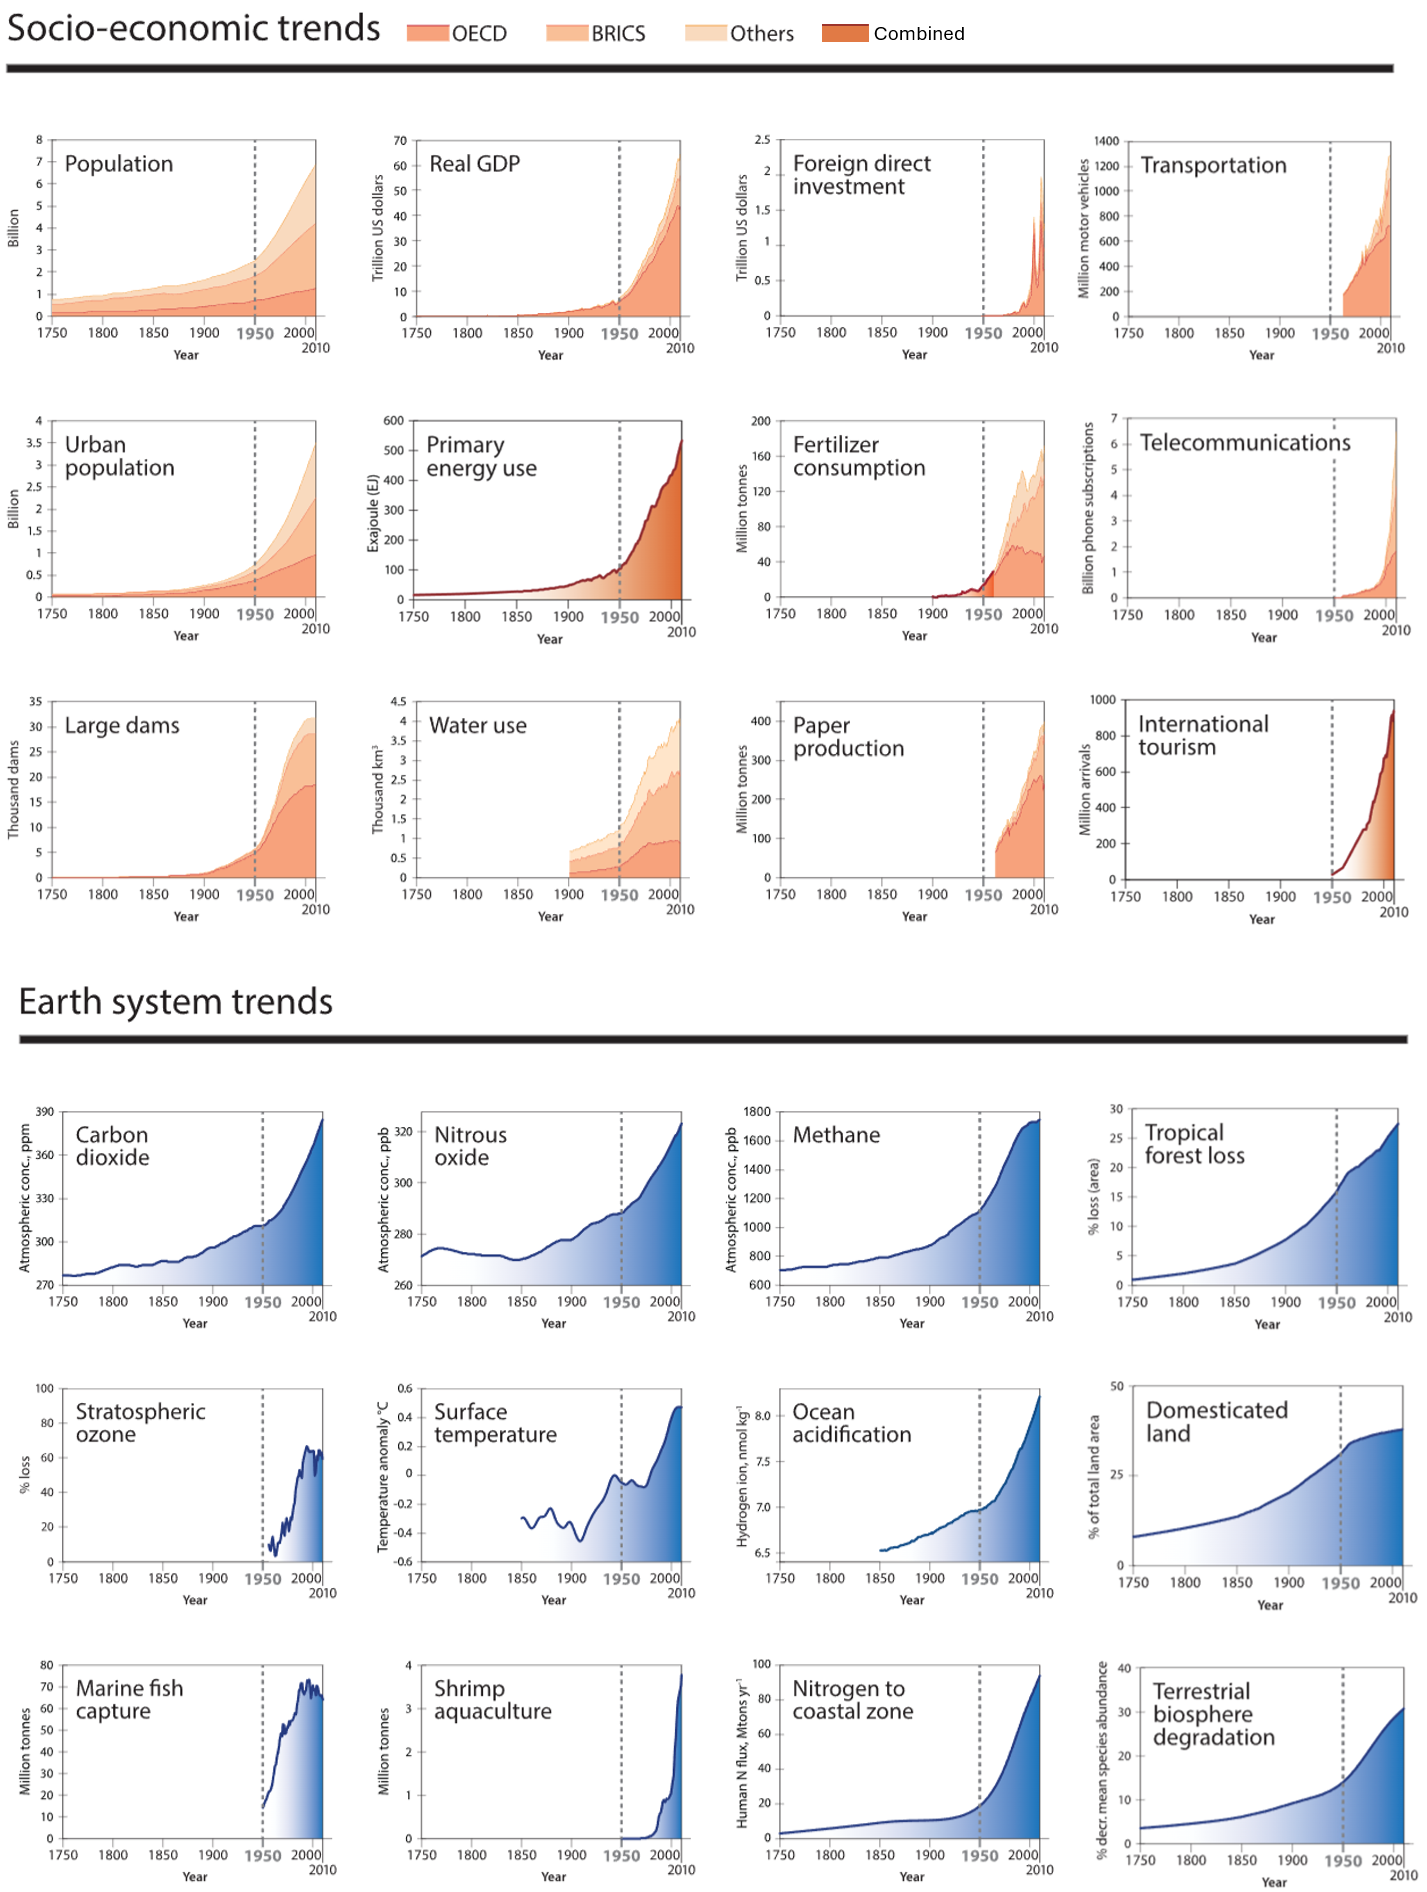
\includegraphics[width=0.97\linewidth]{images/socio_economic_and_earth_system_trends.png}
%     \caption{\small{The Great Acceleration (1750–2010), compact view after Steffen et\,al.\ (2015) \cite{steffen2015trajectory}.  Top: Global socio-economic trends split by OECD, BRICS, and the rest, accelerated post-1950 with sharp growth in population, energy, transport, fertilizer, water, and telecommunications. Bottom: Earth-system trends show increases in atmospheric CO\textsubscript{2}, temperature, tropical forest loss, domesticated land use, ocean acidification, and biosphere degradation. These pathways reduce fire resilience and increase wildfire risk through deforestation, biosphere and atmospheric damage, drier conditions, more fuels, and ignitions. Figure \ref{fig:anthropogenic_climate_change_emergency_fire_index}  links this post-1950 shift to observed and projected increases in global fire weather index.}}
%     \label{fig:socio_economic_and_earth_system_trends}
% \end{figure}


% \begin{figure}[H]
%     \centering
%     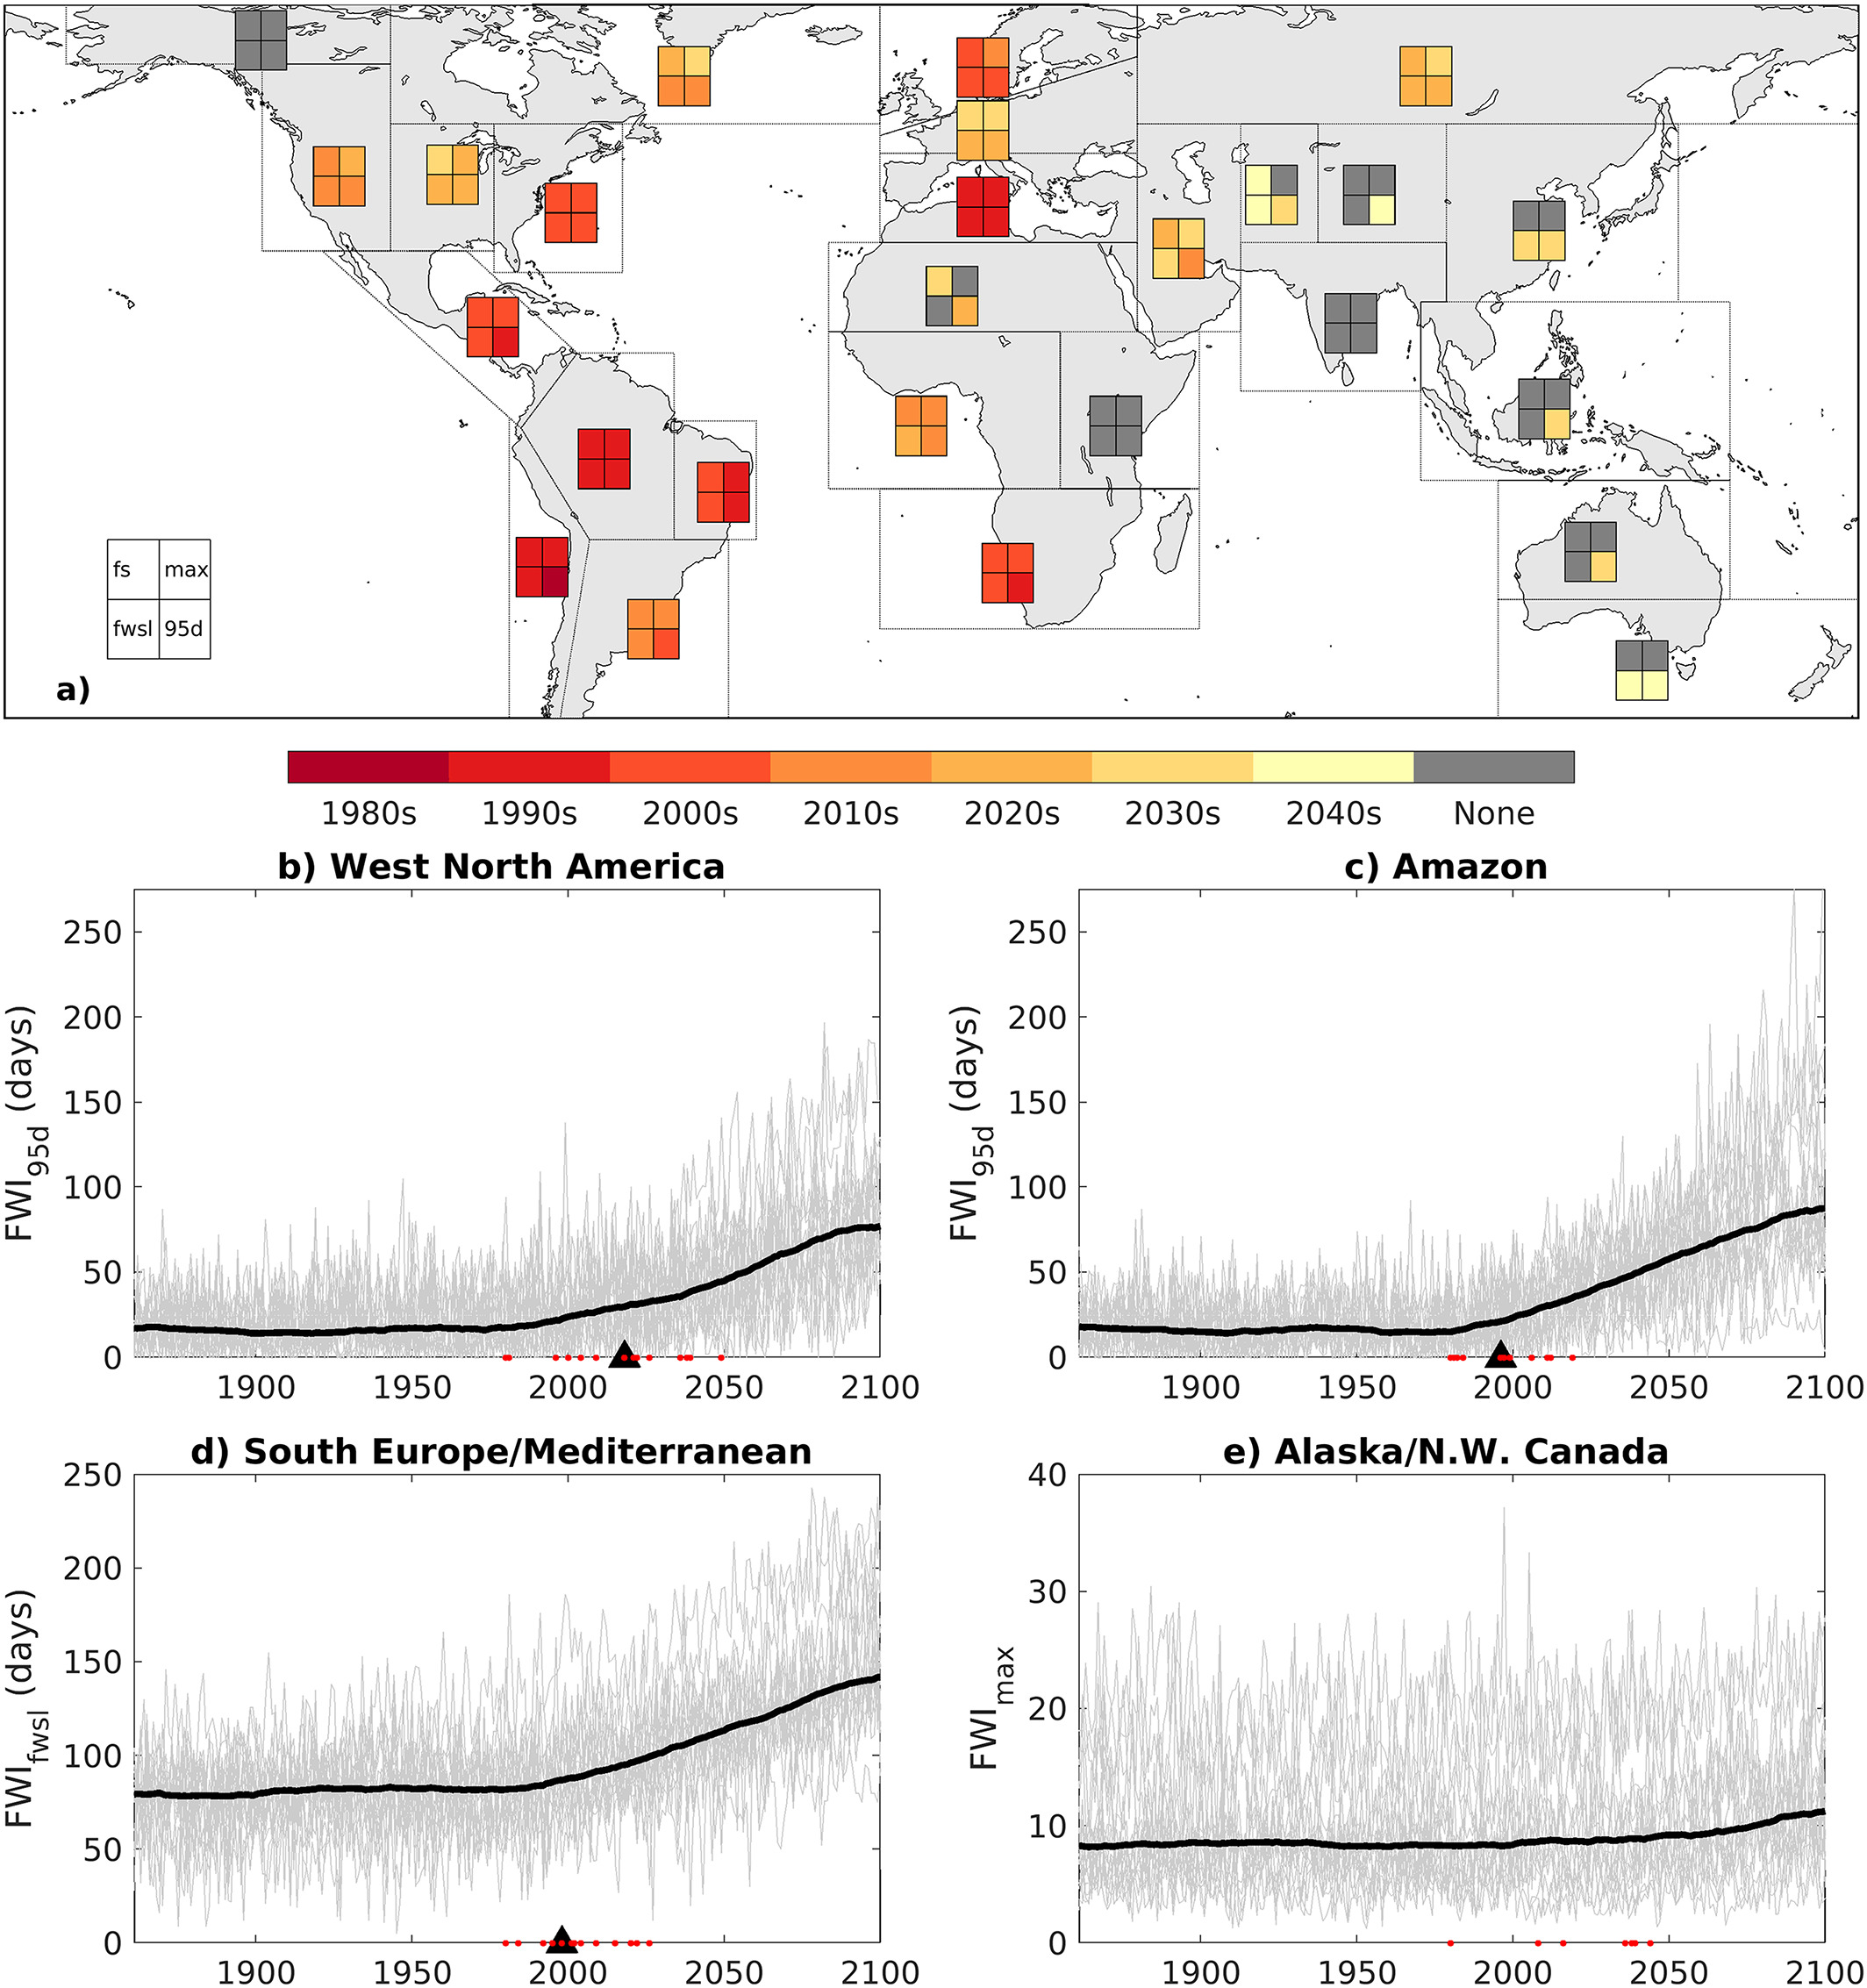
\includegraphics[width=0.95\linewidth]{images/anthropogenic_climate_change_emergency_fire_index.png}

%     \caption{\footnotesize{Time of emergence (ToE) of anthropogenic climate change in Fire Weather Index (FWI) metrics across subcontinental regions.
%     (a) Median ToE from 17 models between (1980-2040); each regional tile shows four metrics by quadrant:
%     95d = FWI$_{95\mathrm{d}}$ (frequency of extreme days),
%     fwsl = FWI$_{\mathrm{fwsl}}$ (season length),
%     fs = FWI$_{\mathrm{fs}}$ (peak 90-day mean),
%     max = FWI$_{\max}$ (annual maximum).
%     Time series between 1861-2100 for selected regions:
%     (b) FWI$_{95\mathrm{d}}$—West North America;
%     (c) FWI$_{95\mathrm{d}}$—Amazon;
%     (d) FWI$_{\mathrm{fwsl}}$—South Europe/Mediterranean;
%     (e) FWI$_{\max}$—Alaska–Northwest Canada.
%     Bold black line: 30-year multimodel median; red dots: each model ToE; black triangle: 17-model median ToE where at least nine models show emergence.
%     \protect\footnotemark}}
%     \label{fig:anthropogenic_climate_change_emergency_fire_index}
% \end{figure}

% \footnotetext{\label{fn:abatzoglou2019}\footnotesize{Reproduced from Abatzoglou, J.~T., Williams, A.~P., \& Barbero, R. (2019), \textit{Geophys. Res. Lett.} 46, 326–336, doi:10.1029/2018GL080959. 
% \copyright~2019 American Geophysical Union.\cite{abatzoglou_global_2019}}}

% \begin{figure}[H]
%     \centering
%     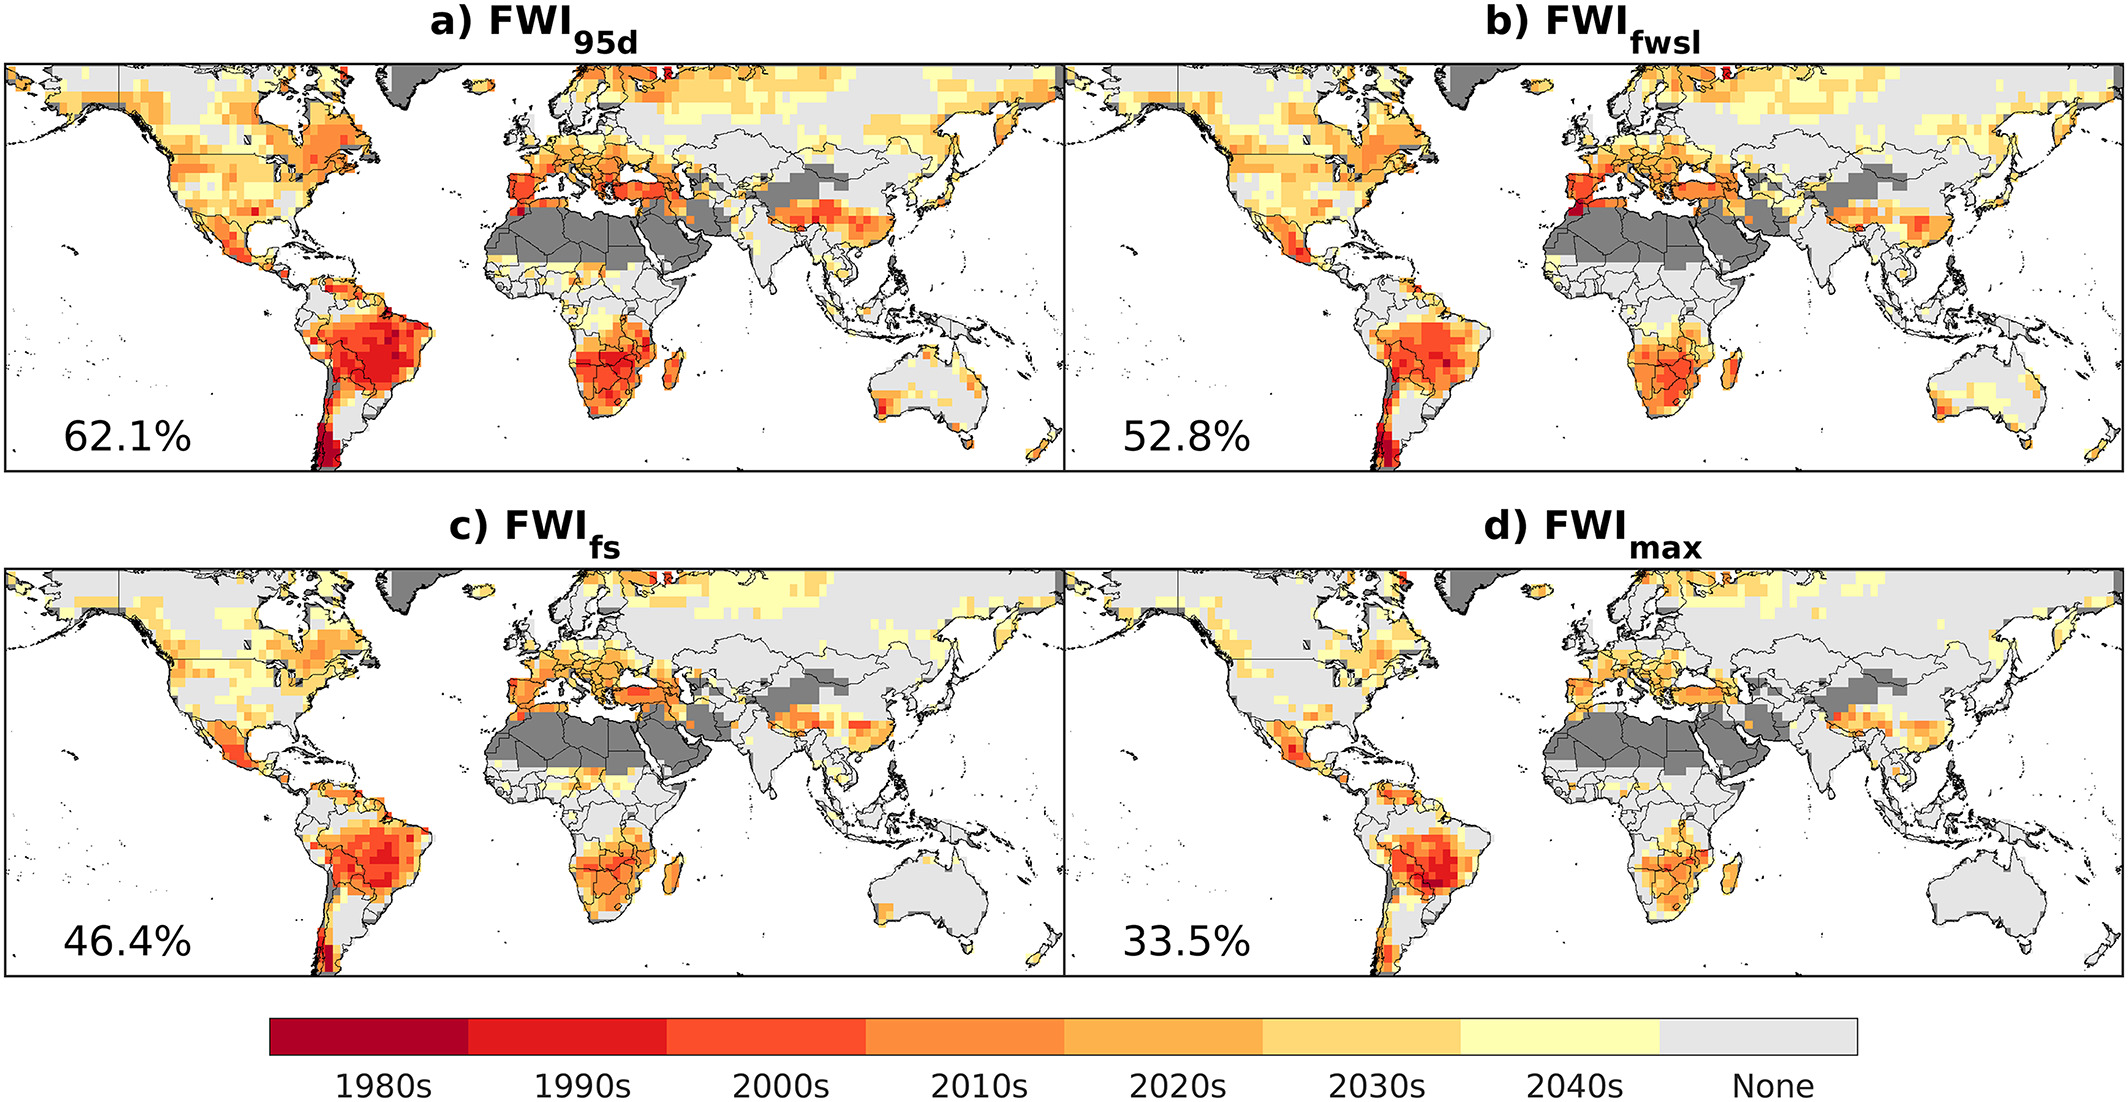
\includegraphics[width=1\linewidth]{images/fire_anthropogenic_ToE_detailled.png}
%     \caption{Time of emergence of anthropogenic climate change for (a) the frequency of days exceeding the 95th percentile (extreme fire days \( \mathrm{FWI}_{\mathrm{95d}} \)), (b) the length of the fire weather season (\( \mathrm{FWSL} \)),(c) the peak 90-day average (FWI$_{\max}$), and (d) annual maximum (\( \mathrm{FWI}_{\mathrm{fs}} \)). Mapped is the 17-model median date at which the anthropogenic signal emerges based on the change exceeding the standard deviation of the baseline period. Areas of light gray highlight where the signal does not emerge for at least eight models by 2050. Unburnable lands where >80\% of the area is water, snow, and ice, or barren or sparsely vegetated, are shown in dark gray. The percent of burnable land with emergence by 2050 is denoted in the bottom left corner of each map.\textsuperscript{\ref{fn:abatzoglou2019}}}
%     \label{fig:anthropogenic_climate_change_emergency_fire_index_detailled}
% \end{figure}

% \subsection{Global Rise of the Fire Weather Index(FWI)}

% Building on climate-model simulations, Abatzoglou et al. (2019) estimate the time at which anthropogenic forcing makes fire-weather indices exceed the range expected from natural variability at subcontinental scales\cite{abatzoglou_global_2019}. Figure \ref{fig:anthropogenic_climate_change_emergency_fire_index}  shows the Time of Emergence (ToE) of anthropogenic climate change in subcontinental regions. 

% The metric used to analyze wildfire risk is the Fire Weather Index (FWI). The FWI is a unidimensional unit that measures the likelihood of fire intensity based on fuel dryness and fire weather, regardless of the type of biomass covering the land. The inputs needed to calculate the FWI are daily temperature, humidity, wind speed, and accumulated rainfall. FWI is explained in more detail in chapter \ref{31-the-fire-itself-physics-of-the-radiative-signature}. The main quantities necessary to understand the fire weather properties used on Figure \ref{fig:anthropogenic_climate_change_emergency_fire_index}- \ref{fig:map_FWSL_FWI95d_change_relative_1979_2019} are summarized in Table \ref{tab:fwi_metrics}.(TODO: Replace table with a drawing of FWI curves connecing the FWI curves and burned areas and fire frequency)

% %\begin{itemize}
% %  \item \textbf{FWI95d (frequency of extreme days).} Number of days per year when daily FWI exceeds the local 95th-percentile threshold defined from a historical baseline; indicates how often “very bad” fire-weather occurs.
% %  \item \textbf{FWIfwsl (fire-weather season length).} Days per year with FWI above the mid-range point (average of the local baseline maximum and minimum FWI); indicates how long conditions remain conducive to fire spread.
% %  \item \textbf{FWIfs (seasonal peak 90-day severity).} Highest 90-day running mean FWI within the year; captures the intensity of the core fire season regardless of its timing.
% %  \item \textbf{FWImax (annual daily maximum).} Single highest daily FWI in the year; a magnitude-of-extremes metric related to the potential for extreme runs/spread.
% %\end{itemize}


% \begin{table}[h]
% \centering
% \footnotesize
% \begin{tabularx}{\textwidth}{|l|l|X|}
% \hline
% \textbf{Symbol} & \textbf{Meaning} & \textbf{Description} \\
% \hline
% $\mathrm{FWI}$ & Fire weather index & 
% Unitless composite from daily max temperature, min relative humidity, 24\,h precipitation, and mean wind speed; combines fuel-moisture buildup and wind-driven spread. \\
% \hline
% $\mathrm{FWI}_{95\mathrm{d}}$ & Extreme days per year & 
% Number of days in a year when daily FWI exceeds the local 95th-percentile threshold (threshold from a historical baseline). \\
% \hline
% $\mathrm{FWI}_{\mathrm{fwsl}}$ & Season length & 
% Days per year with FWI above the mid-range point (average of the local baseline maximum and minimum FWI). \\
% \hline
% $\mathrm{FWI}_{\mathrm{fs}}$ & Peak 90-day severity & 
% Highest 90-day running mean FWI within the year (sliding window), capturing core-season intensity regardless of timing. \\
% \hline
% $\mathrm{FWI}_{\max}$ & Annual maximum & 
% Maximum daily FWI observed in the year (single-day extremity). \\
% \hline
% \end{tabularx}
% \caption{Fire Weather Index (FWI) metrics used in wildfire risk assessment}
% \label{tab:fwi_metrics}
% \end{table}


% Abatzoglou et al.\cite{abatzoglou_global_2019} report that anthropogenic effects on fire weather index signals are detectable with increased amplitude in parts of southern Europe, West Noth America, South African Savannahs, the Amazon, and other regions. We can analyze the historical anthropogenic FWI effect by verifying the high-level Figure \ref{fig:anthropogenic_climate_change_emergency_fire_index}-a and the low-level detailed Figure \ref{fig:anthropogenic_climate_change_emergency_fire_index_detailled}. These plots show the Time of Emergence (ToE) of the anthropogenically induced FWI in different points for each sub-continent region. The earliest observable effect starts in the 80s, in the Peruvian Amazonian/Chile region. Between the 90s and 00s, we see a large emergent impact covering the Amazon, South Europe/Mediterranean, Northern Europe, Central America, Northeast and South Brazil, Argentina, the South African region, and Eastern North America. Later, between 10s-20s, human impact appears in Central and West North America, the North Canada/Greenland tundra region, central and north Africa, Western Asia, and Western and Eastern Europe. The prediction for anthropogenic fire activity impact extended between 30s-40s, where effects are seen in Western and Eastern Asia, South-eastern Asia, and Australasia. 

% Detailed trend of the fire weather season length \( \mathrm{FWSL} \)  and extreme fire days \( \mathrm{FWI}_{\mathrm{95d}} \) per region is seen in Fig \ref{fig:fire_season_FWSL_1979_2019} and Fig \ref{fig:fire_extreme_days_freq_FWSI95d_1979_2019}. Analyzing first the season length Fig \ref{fig:fire_season_FWSL_1979_2019},  in this plot, one can see that globally the fire season length increases from \(\sim\)60 days (2025) to \(\sim\)70 days (2050) and \(\sim\)78 days (2100). These values are a global average; however, it is important to note the regions where planetary frontiers can be crossed, and where human and biome life will be affected more severely and sooner. One region identified as a planetary tipping point that must keep fire weather under control to prevent a planetary critical transition is the Amazon. From Figure \ref{fig:fire_extreme_days_freq_FWSI95d_1979_2019} the Amazon extreme fire weather days per year \( \mathrm{FWI}_{\mathrm{95d}} \) goes from about 25 days in 2025 to approximately 50 days in 2050, and about 100 days in 2100. This increase in wildfire activities is likely linked to the deforestation–drought–fire feedbacks and could signify the savannization of the Amazonian biome, which aligns with tipping points and critical transitions. scenarios.(TODO:Mission requirement def, Secondary coverage, Amazon critical parts).\footnote{Rising fire-weather pressure in the Amazon interacts with deforestation–drought–fire feedbacks that may push parts of the biome toward "savannization." Multiple assessments place a tipping threshold near $\sim$20–25\% cumulative deforestation; The full Amazon forest basin loss has been reported at $\sim$17\% (and nearing 20\% in Brazil), showing the narrowing margin \cite{lovejoy_amazon_2019}. Regional research consortia warn this threshold could be approached in the 2025–2030 window under high-loss trajectories \cite{raisg_against_clock_2022}, while a recent \textit{Nature} synthesis projects that by $\sim$2050, 10–47\% of Amazon forests could face compounding disturbances capable of triggering local-to-regional transitions \cite{flores_critical_2024}. Within the Planetary Boundaries lens, these dynamics reflect interacting transgressions of land-system change and biosphere integrity, amplifying fire-weather risks \cite{richardson2023earth}.}

% Although impacts in the Amazon have planetary consequences in human population and biosphere/biodiversity, the most severe \textit{projected} increases in fire-weather exposure occur over southern Europe/the Mediterranean (Fig.~\ref{fig:anthropogenic_climate_change_emergency_fire_index}d), where the fire-season length metric \( \mathrm{FWSL} \) rises from \(\sim\)90 days (2025) to \(\sim\)120 days (2050) and \(\sim\)150 days (2100). Additionaly, Fig \ref{fig:fire_extreme_days_freq_FWSI95d_1979_2019} shows that the Mediterranean extreme fire days  \( \mathrm{FWI}_{\mathrm{95d}} \) increase from  \(\sim\)30 days (2025) to \(\sim\)45 days (2050) and \(\sim\)75 days (2100). Beyond wildfire meteorology, this region is a warming–aridification hotspot with large and dense connected wildland–urban interface and land-use legacies that amplify ignitions and losses. (TODO:Mission requirement def, Primary sub-continental region good for fast wildfire detection)(TODO: talk about the increase of death due to heatwaves)

% A planetary vision under the metric of the fire weather season length, which measured the impact of natural and anthropogenic causes of fire between 1979 and 2019, is projected onto the global map Fig \ref{fig:map_FWSL_FWI95d_change_relative_1979_2019}. 

% A planetary vision under the metric of the fire‐weather season length, which measured the impact of natural and anthropogenic causes of fire between 1979 and 2019, is projected onto the global map in Fig.~\ref{fig:map_FWSL_FWI95d_change_relative_1979_2019}. As analyzed by Jones et. al, on this plot, we see a synthesis of the trends under discussion; it's possible to see a crescent trend for the \( \mathrm{FSWL} \) and \( \mathrm{FWI}_{\mathrm{95d}} \). Also, as these metrics grow at different rates— in South America, Central Asia, and Africa, the increase in extreme days per year was greater than the expansion of the fire season length. On the other hand, in Europe and boreal Asia, the growth of the season was larger than the increase in extreme days.  The places with the earliest anthropogenic fire impact are the ones with the largest change in the relative fire season length, namely, Europe, central and boreal Asia, southern‐hemisphere South America, and temperate North America. Regarding the extreme fire days per year, the highest increase is in southern‐hemisphere South America, central Asia, and across Africa\cite{jones_global_2022}.

% \begin{figure}[H]
%     \centering
%     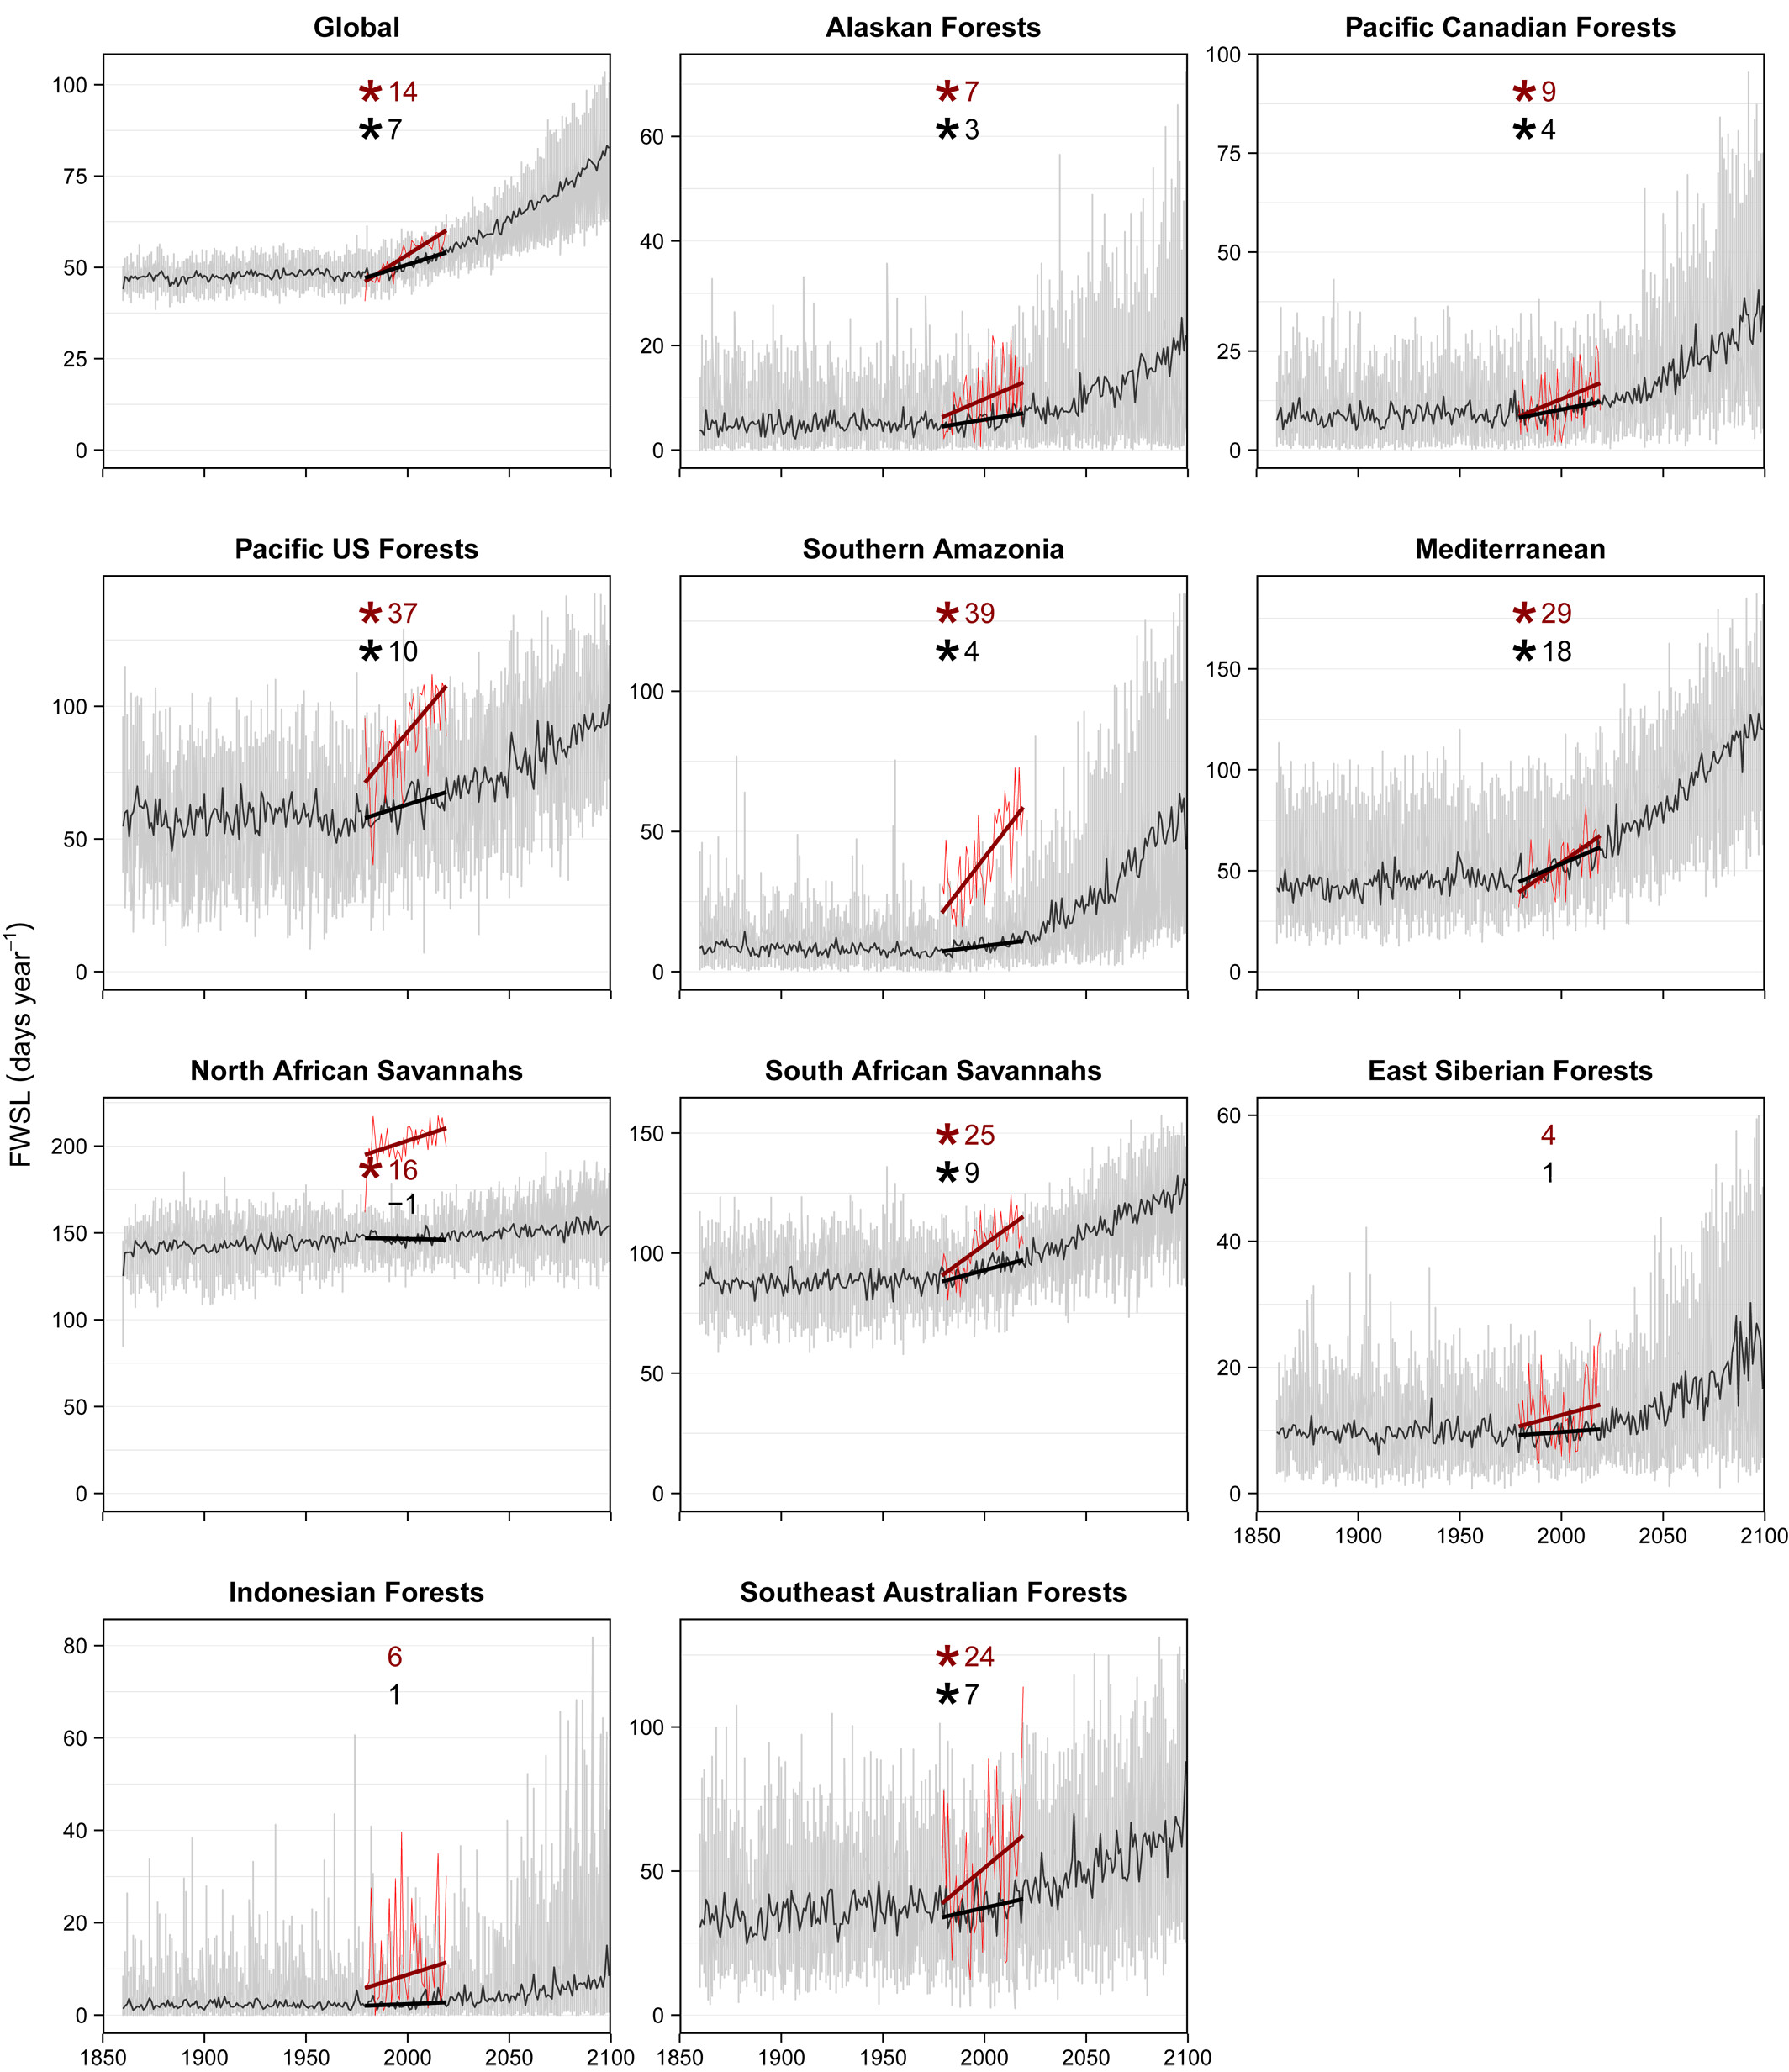
\includegraphics[width=0.95\linewidth]{images/FWSL_region_comparation.png}
%     \caption{\footnotesize{Time series of global and regional estimates of mean fire weather season length (FWSL) from measurements analyzed by ERA5 (thin red lines; Hersbach et al.,[2020]; Vitolo et al., [2020] and CMIP5 models running RCP8.5 (gray lines; Abatzoglou et al., [2019]. Thin black lines mark the multi-model mean estimate from the CMIP5 models. Linear trends in the period 1979–2019 are shown for the ERA5 (thick red lines) and CMIP5 (thick black lines), with corresponding numbers marking the change in annual FWSL during the period (the slope integrated over the period 1979–2019) and corresponding asterisks denoting significant changes at the 95\% confidence interval. Differences between modeled and observed FWSL can be explained by differences in the resolution of the models (2.5°) versus the observations (0.25°), since FWSL is partly determined by the maximum value FWI and this is reduced through spatial averaging.\protect\footnotemark}}
%     \label{fig:fire_season_FWSL_1979_2019}
% \end{figure}
% \footnotetext{\label{fn:jones2022}\footnotesize{Reproduced from Jones \emph{et al.} (2022), \cite{effisPRTstats}. Licensed under \href{https://creativecommons.org/licenses/by/4.0/}{CC BY 4.0}.}}

% \begin{figure}[H]
%     \centering
%     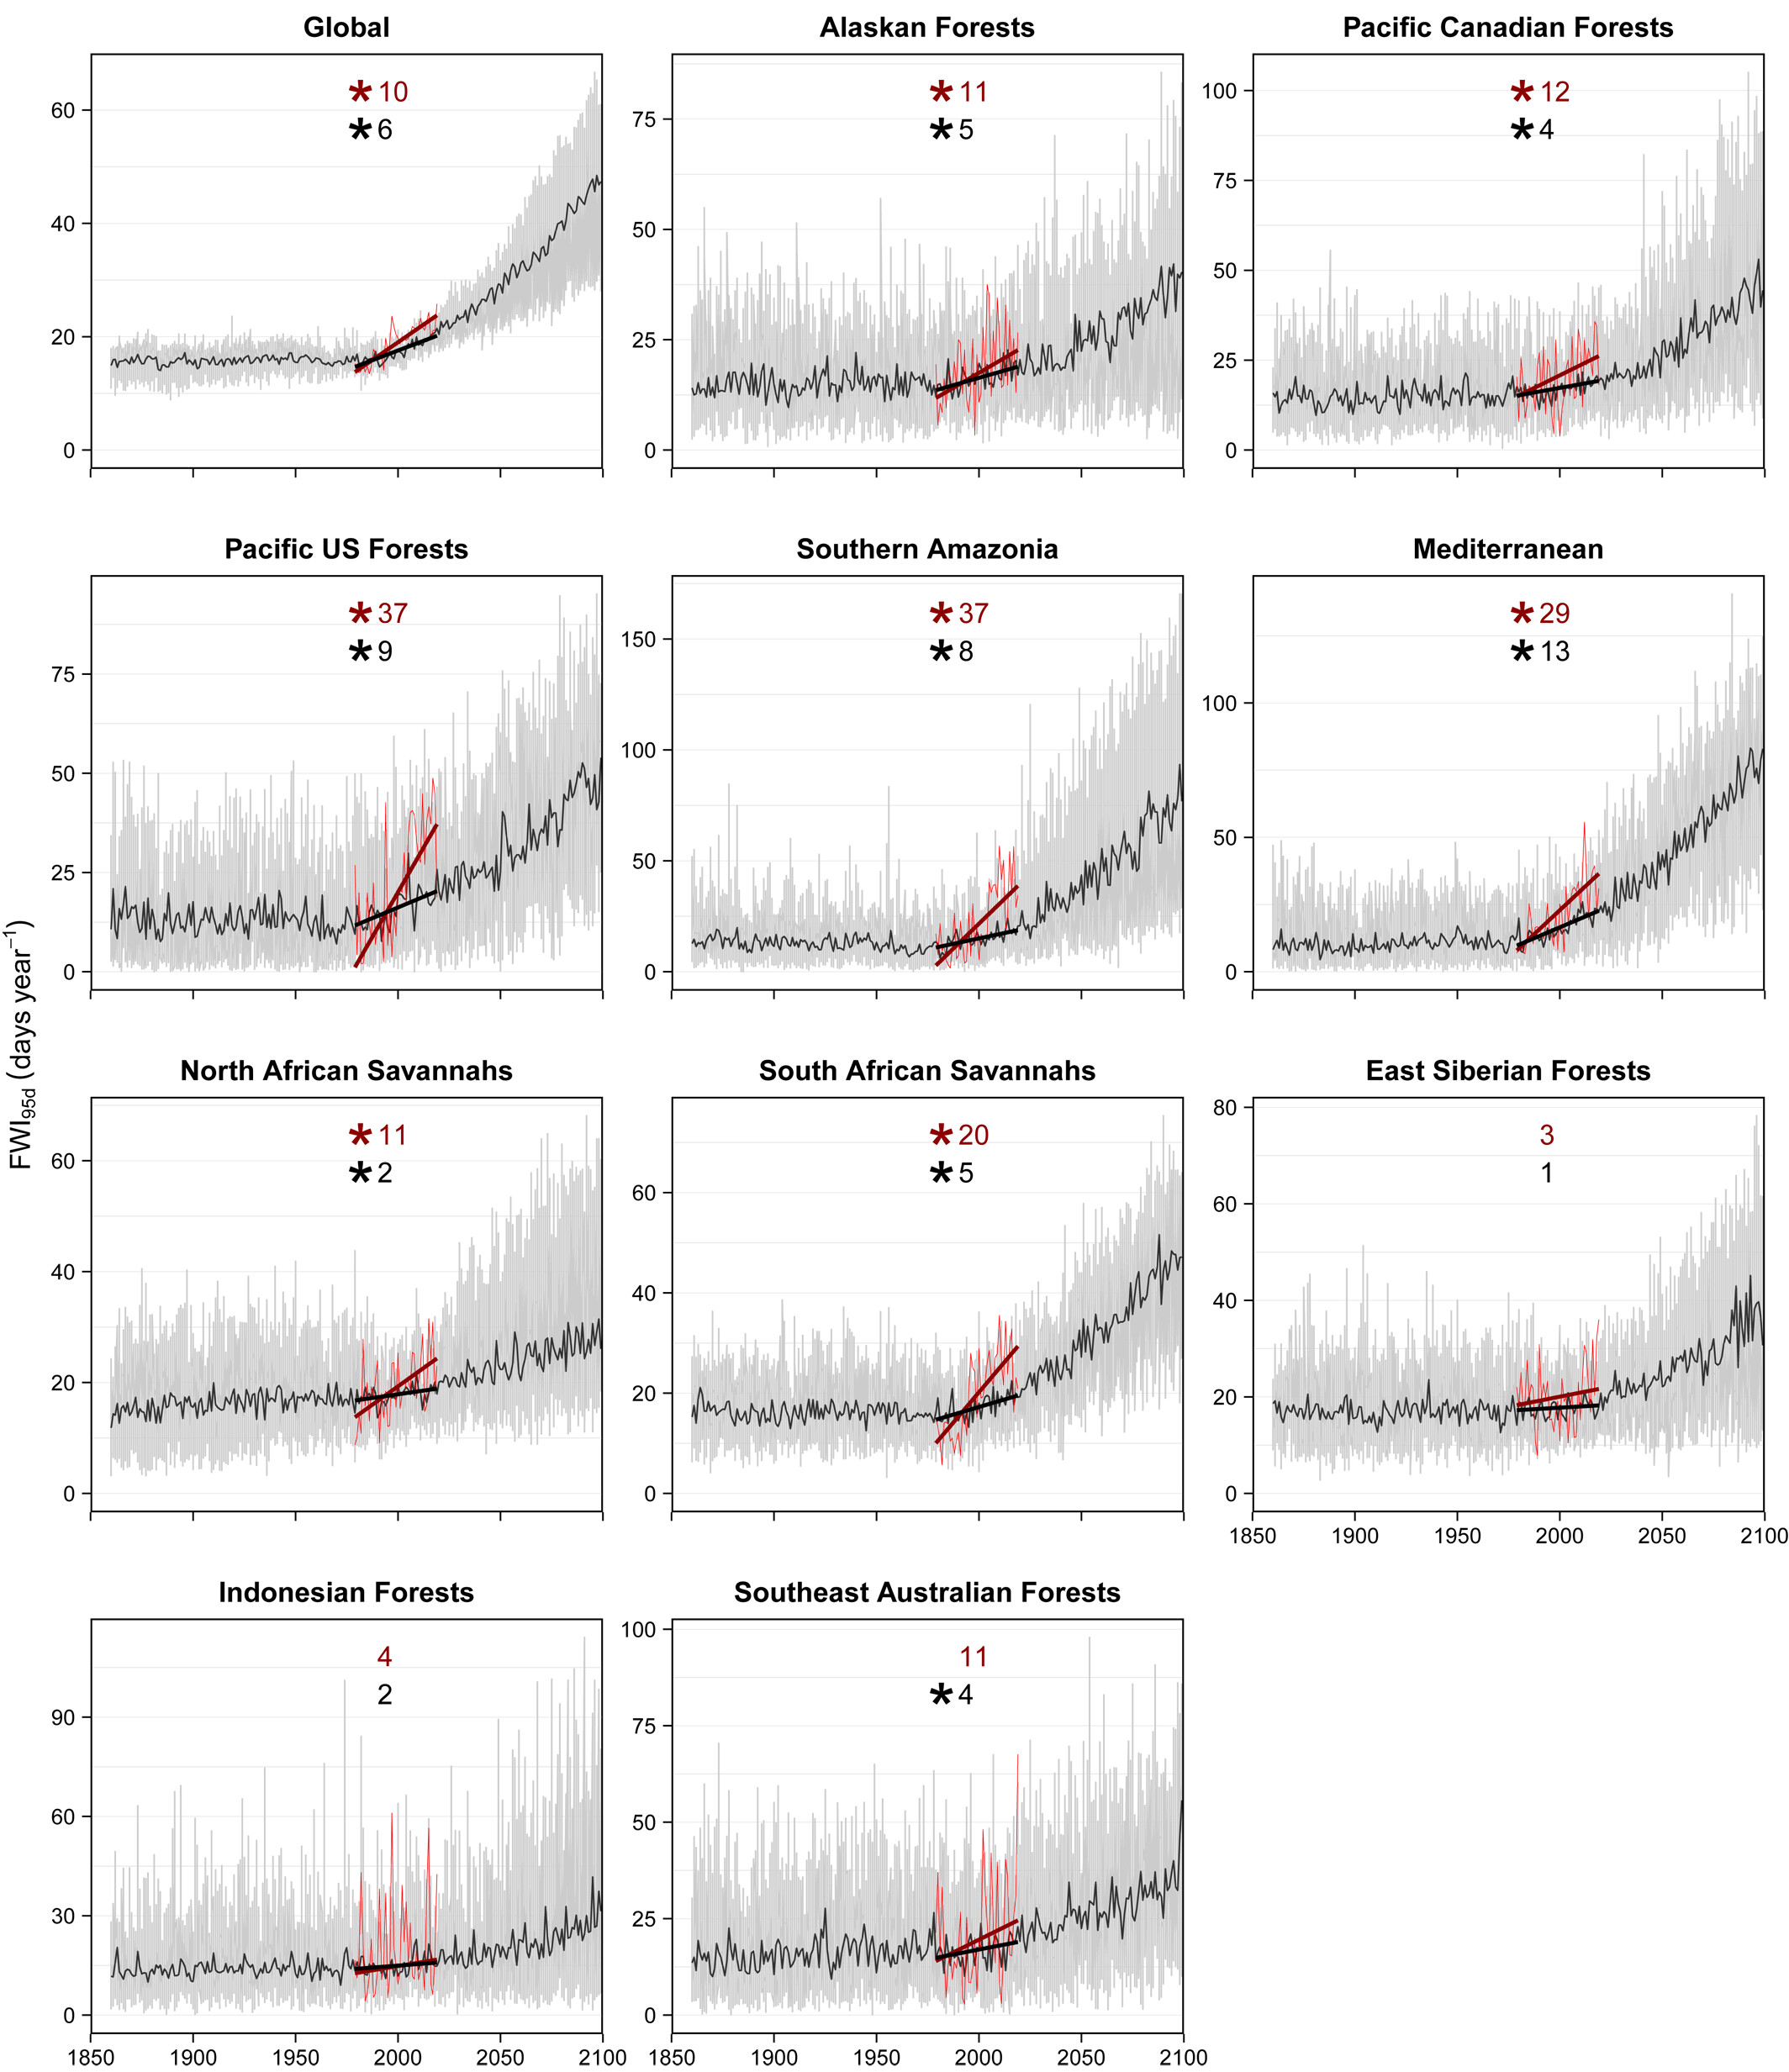
\includegraphics[width=1\linewidth]{images/region_comparation_fire_index.png}
%     \caption{Time series of global and regional estimates of mean FWI95d from ERA5 (thin red lines; Hersbach et al., 2020; Vitolo et al., 2020) and CMIP5 models running RCP8.5 (gray lines; Abatzoglou et al., 2019). Thin black lines mark the multi-model mean estimate from the CMIP5 models. Linear trends in the period 1979–2019 are shown for the ERA5 (thick red lines) and CMIP5 (thick black lines), with corresponding numbers marking the change in annual FWSL during the period (the slope integrated over the period 1979–2019) and corresponding asterisks denoting significant changes at the 95\% confidence interval.\textsuperscript{\ref{fn:jones2022}}}
%     \label{fig:fire_extreme_days_freq_FWSI95d_1979_2019}
% \end{figure}

% \begin{figure}[H]
%     \centering
%     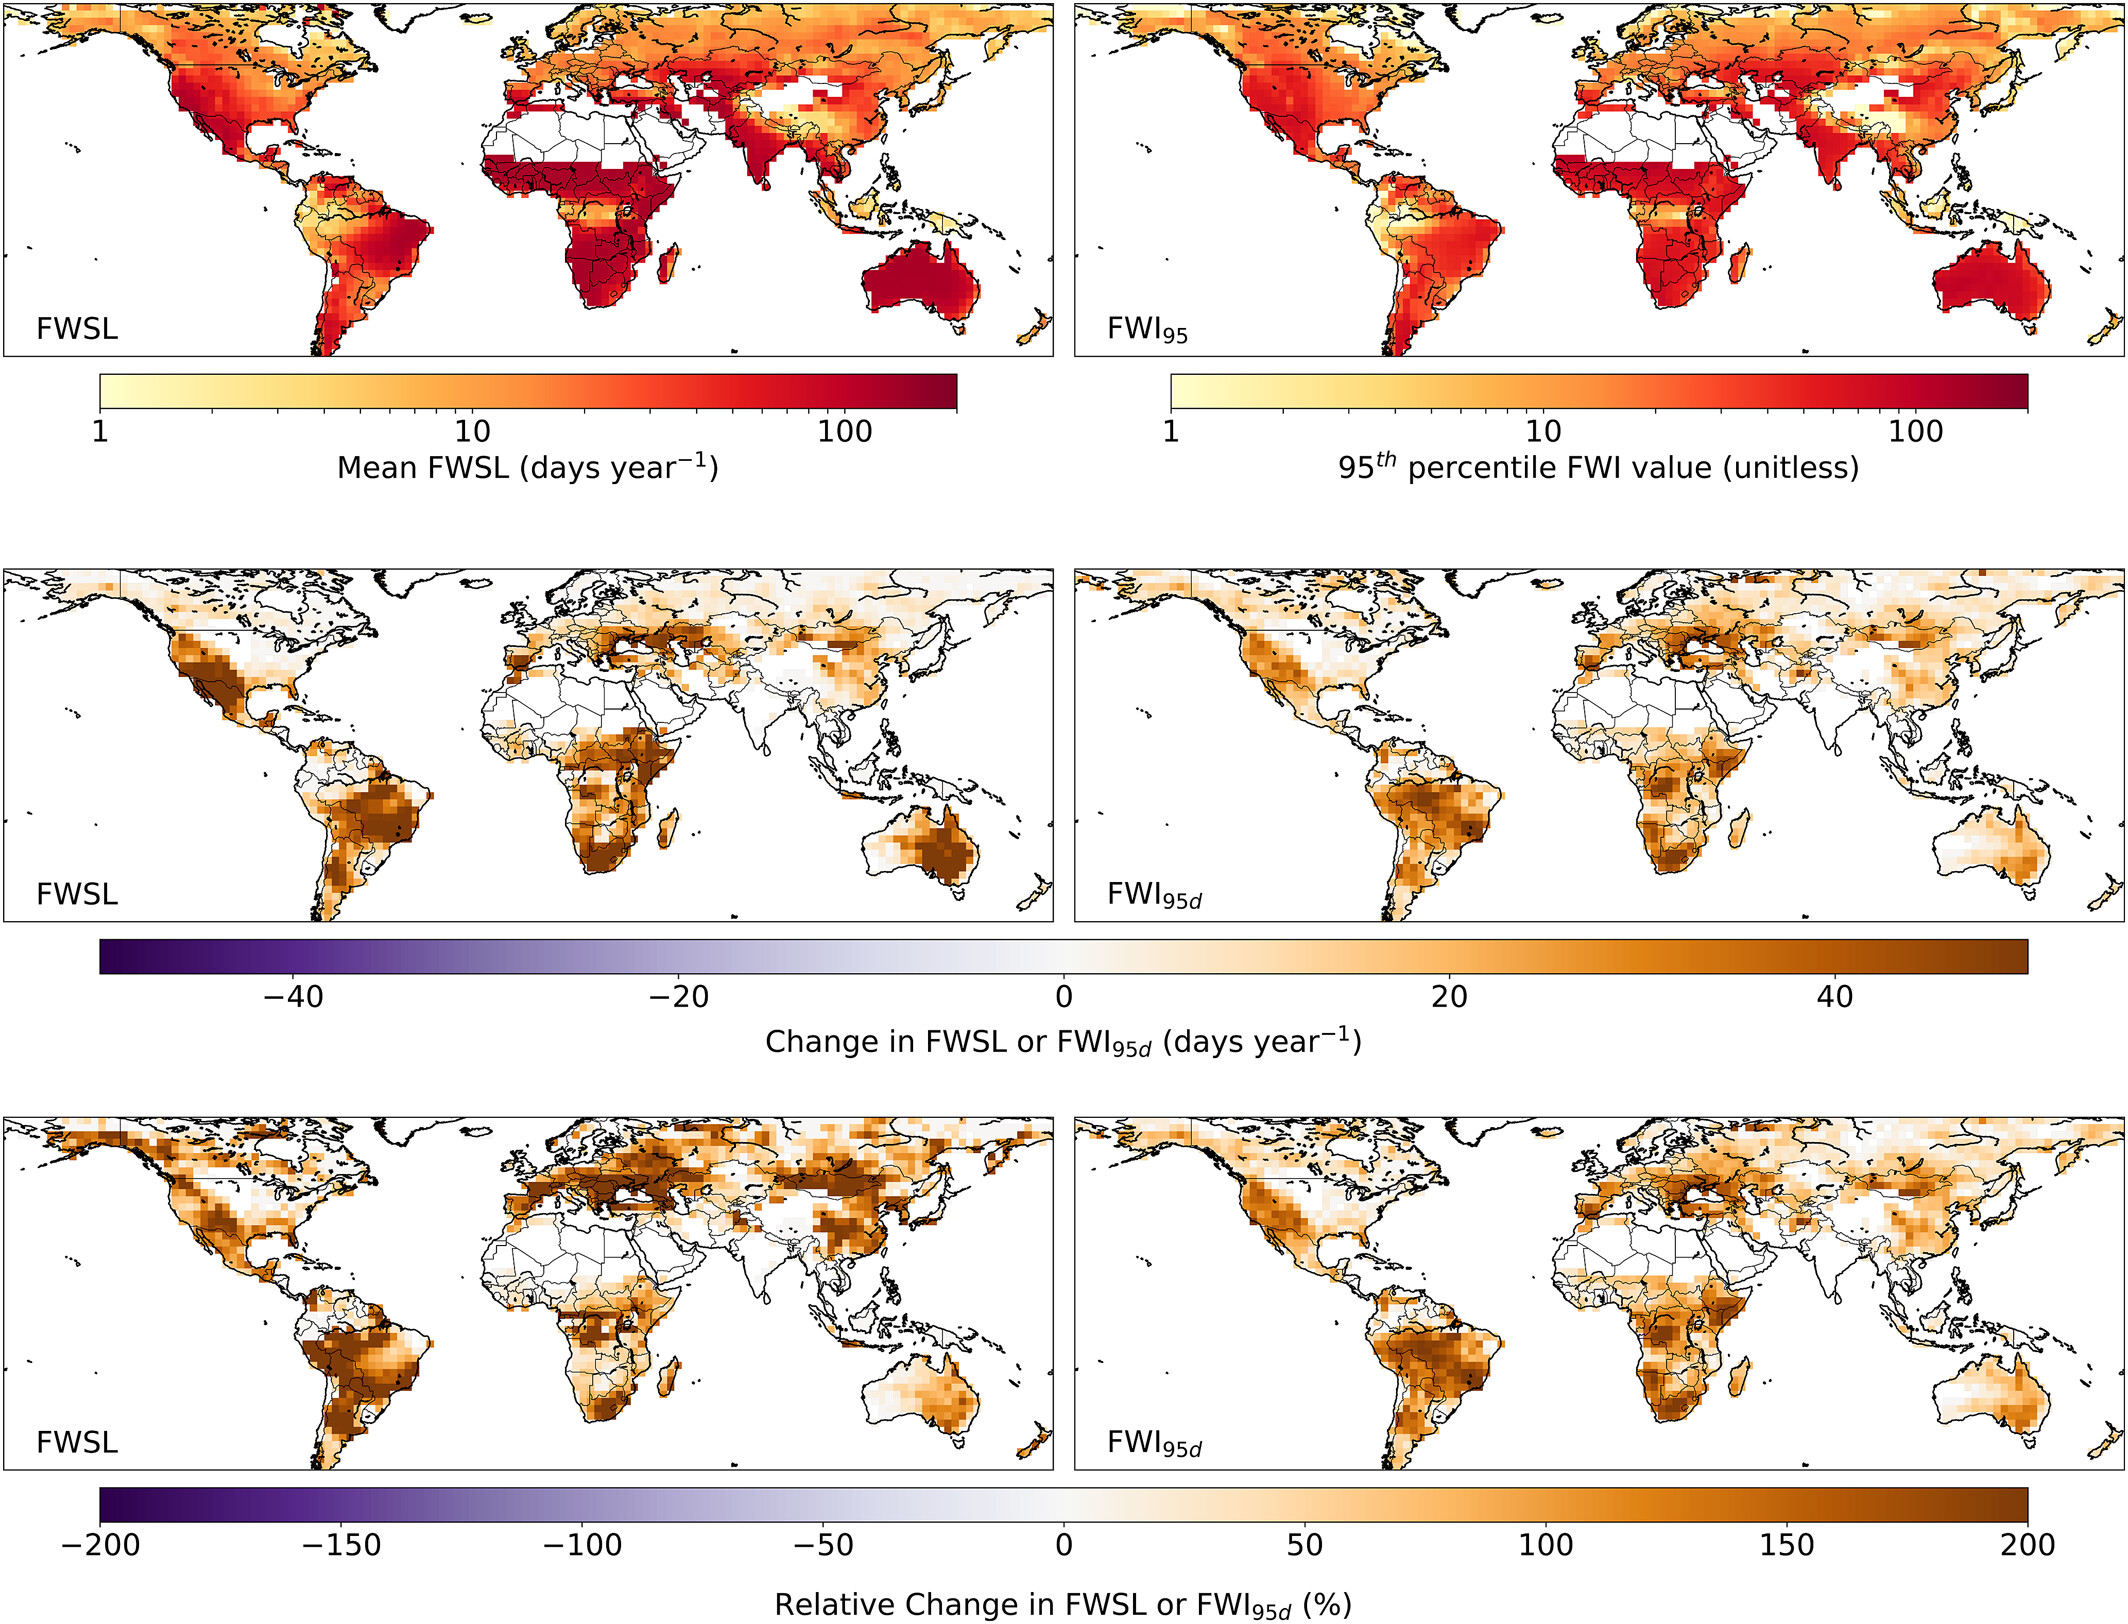
\includegraphics[width=1\linewidth]{images/FWSL_FWI95d_1979_2019_mean_absolute_relative.png}
%     \caption{Global patterns and trends in fire weather during 1979–2019 based on ERA5 reanalysis data (Hersbach et al., [2020]; Vitolo et al., [2020]. (Left panels) include (top) mean, (middle) absolute change and (bottom) relative change in annual fire weather season length (FSWL) during 1979–2019. (Right panels) include (top) the 95th percentile daily value of fire weather index (FWI) threshold value during 1979–2019, (middle) the absolute change in annual days with FWI values exceeding the 95th percentile and (bottom) the relative change. Absolute change (days year−1) is calculated as the trend (days year−2) multiplied by the length of the time series (41 years). The relative change is the absolute change divided by the mean.\textsuperscript{\ref{fn:jones2022}}}
%     \label{fig:map_FWSL_FWI95d_change_relative_1979_2019}
% \end{figure}

% \begin{figure}[H]
%     \centering
%     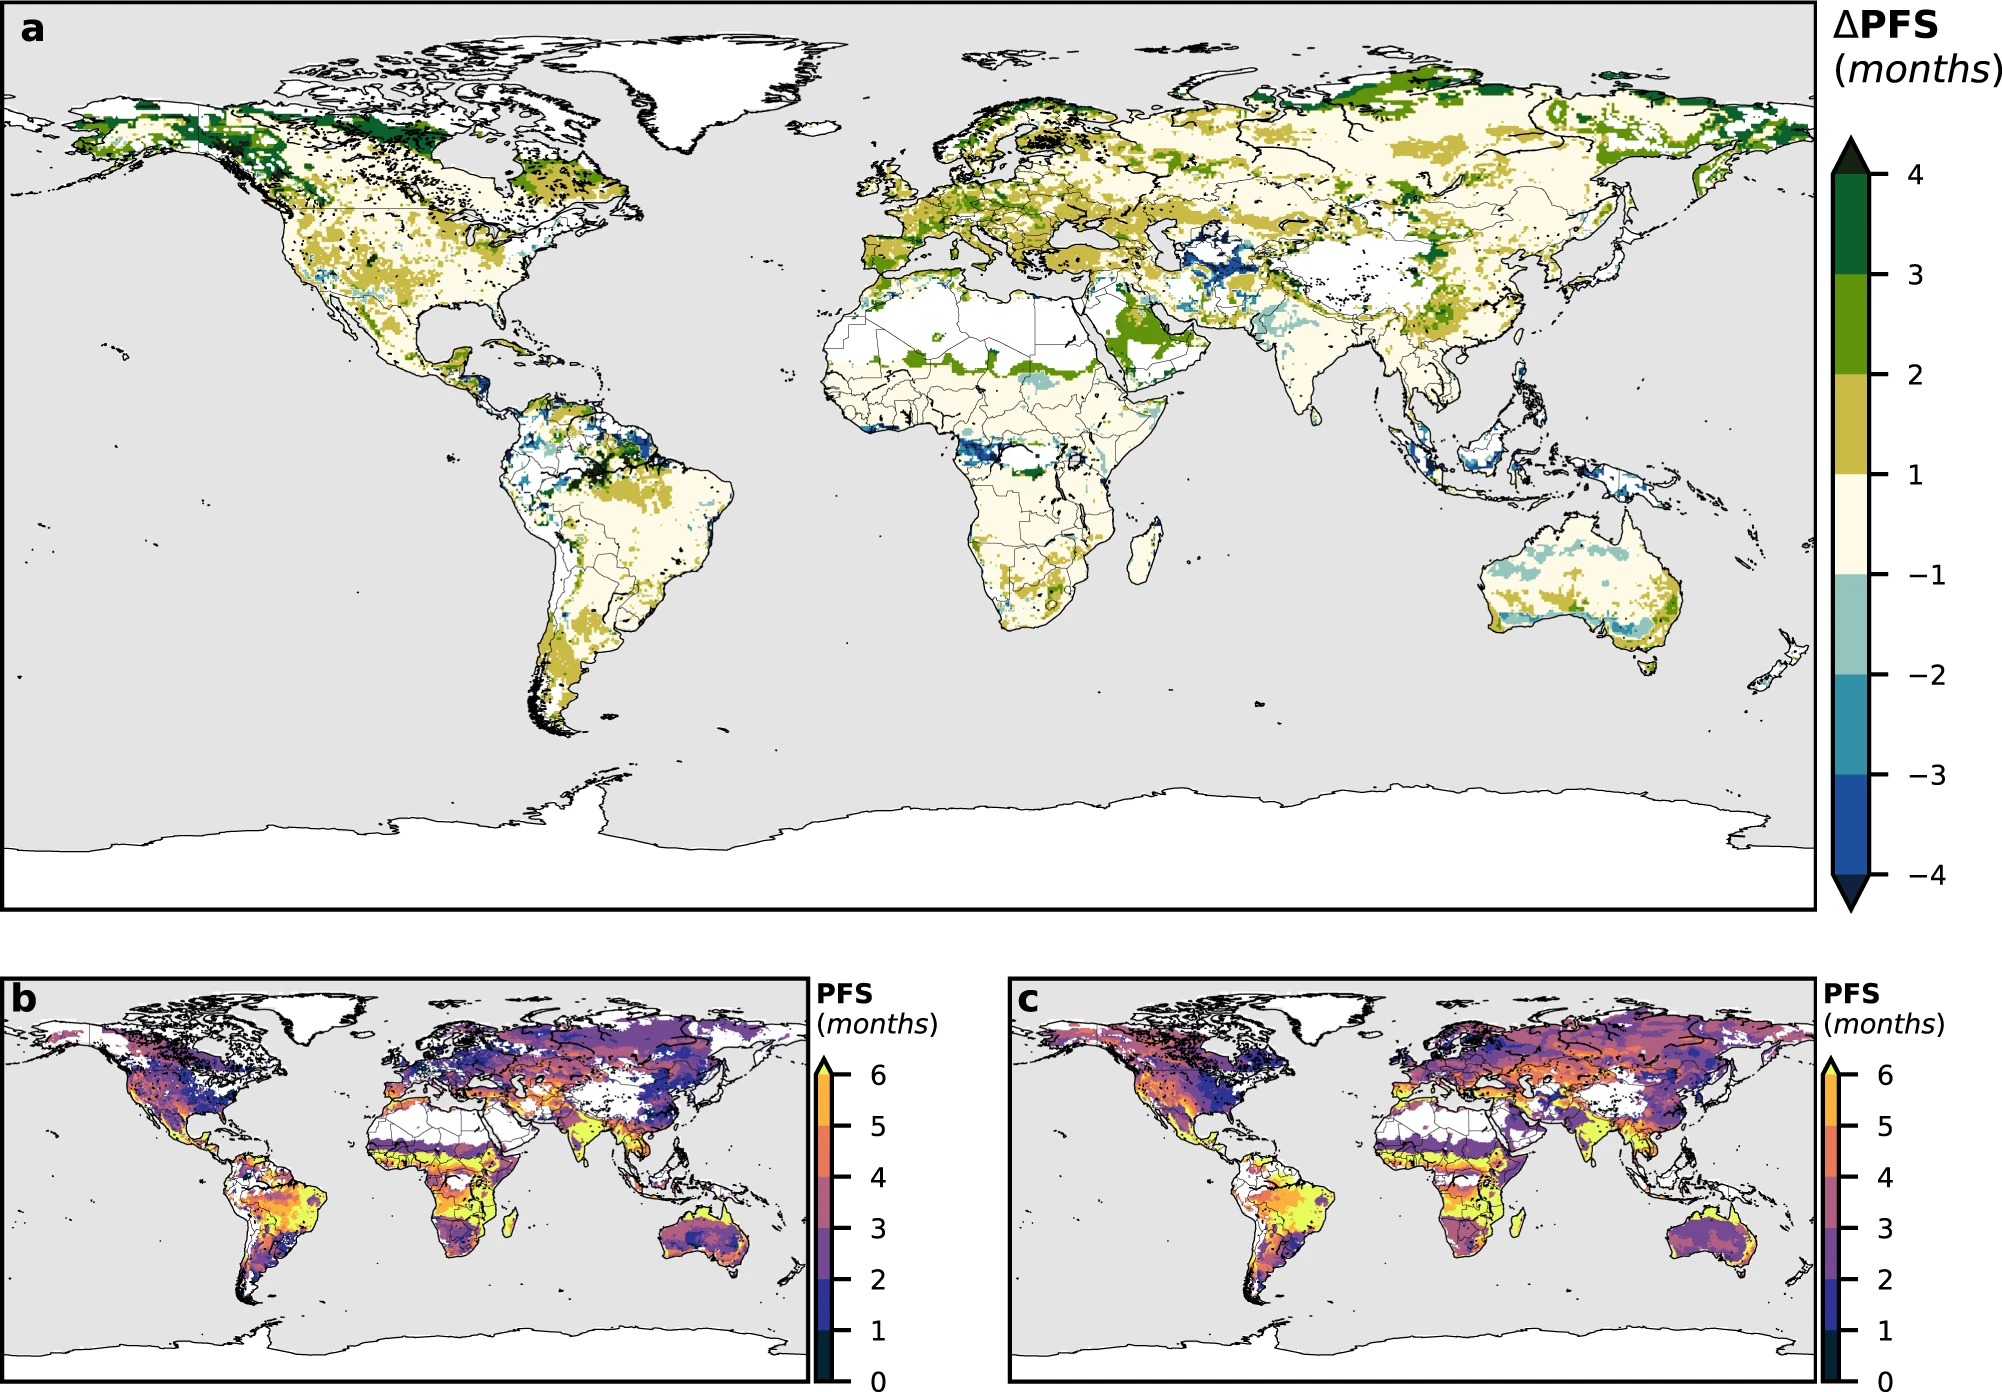
\includegraphics[width=1\linewidth]{images/fire_season_global_change_future_present.png}
%     \caption{(TODO:Add this analysis) a Future minus present potential fire season length (PFSL) difference in months (ΔPFSL). b Present potential fire season. c Future potential fire season.https://www.nature.com/articles/s41467-022-28835-2/figures/3}
%     \label{fig:fire_season_global_change_future_present}
% \end{figure}

% \begin{figure}[H]
%     \centering
%     \includegraphics[width=1\linewidth]{images/map_prediction_dT4_FWSL_FWI.png}
%     \caption{Enter Caption}
%     \label{fig:map_prediction_dT4_FWSL_FWI}
% \end{figure}

% \paragraph{Conclusion.}
% Taken together, the Great Acceleration framing and multi-model fire-weather diagnostics indicate that anthropogenic forcing has already emerged in regional fire climates and is lengthening the window of high-risk conditions while increasing the frequency of extreme fire-weather days \cite{steffen2015trajectory,abatzoglou_global_2019,jones_global_2022}. These signals are especially pronounced in Mediterranean-type climates and across key tropical biomes, where land-use legacies and expanding wildland–urban interfaces amplify ignition pressure and losses. In practical terms, if biomass as fuel is available, the climate crisis is converting more days into days when fires start faster, spread farther, and are harder to control. This establishes the operational need that motivates the present work: a high-temporal, sufficiently resolved, low-latency orbital sensing capability that can shorten detection and modeling feedback loops. The next subsections therefore narrow from the global picture to Portugal—situated within a Mediterranean hotspot—to articulate why current, low-revisit imagery is mismatched to the new hazard regime and how a dedicated constellation can enable earlier detection, better spread forecasts, and more effective firefighting.




% \subsection{Burned Area Trends}

% \subsubsection{Decreasing in Global Burned Area}

% Although the past, present, and future Fire Weather Index (FWI) predictions are important for indicating fire danger in a specific spacetime region on Earth, the FWI alone does not measure fire activity or the actual damage caused to the environment. By managing the availability of flammable biomass, a region with high FWI danger may have a null Burned Area (BA) without destruction. Therefore, the \textit{metric that truly measures fire damage is the BA}.

% Before the advent of Earth observation satellites, historical series measurements of BA on a global scale were neither accurate nor readily accessible. The 1960s and 1970s marked the beginning of spaceborne BA measurements. Consequently, to estimate BA future or past trends, simulation models were developed based on the BA satellite-observation database. 

% A modern example of a BA model is the Fire Model Intercomparison Project (FireMIP), which is a combination of X models.  On Fig \ref{fig:regional_series_fireMip} we can see FireMIP BA analysis between 1900-2020. On this plot, the Global BA matches closely the FireMip\textbf{ median BA prediction of ~\(4.3 \times 10^{6}\ \mathrm{km^{2}\,yr^{-1}}\)  on the period between 2000 an 2015}. During this temporal interval, it is possible to observe a \textbf{global decreasing trend in BA }not only in the model prediction, but also in the observed satellite data of MODIS (red line). 
% A detailed BA trend of the same period was also conducted by Giglio et al., and it is shown in Fig  \ref{fig:BA_global_trend_regions}. This plot displays a \textbf{global decreasing trend in BA aproximately \(-1.1 \times 10^{6}\ \mathrm{km^{2}\,}\) per year.} \textbf{(Giglio et al. 2018 - MISSING CITATION)}. Besides BA model trends, Andela et al. (2017) used satellite data to create a visualization of the observed BA from satellites, which is shown in Fig. \ref{fig:map_BA_global_decrease_1998_2015}. This study confirms the decreasing global trend, with a measured \textbf{decline in BA of -24.3 ± 8.8\% between 1998 and 2015}.

% Considering the rise in global temperatures, the increasing impacts of the climate crisis, and the longer, more intense fire seasons, this reduction in the global BA trend is unexpected. This paradox is interpreted by Jones et al. (2022) as a "global BA decline since 2001 driven primarily by large reductions of BA in African savannas, where land-use change (cropland expansion, livestock grazing, fragmentation, and enhanced suppression), and regionally reduced vegetation productivity under drier hydrological conditions that limited fuel and fire spread, decoupling burned area trends from the concurrent increases in fire weather index.”

% \begin{figure}
%     \centering
%     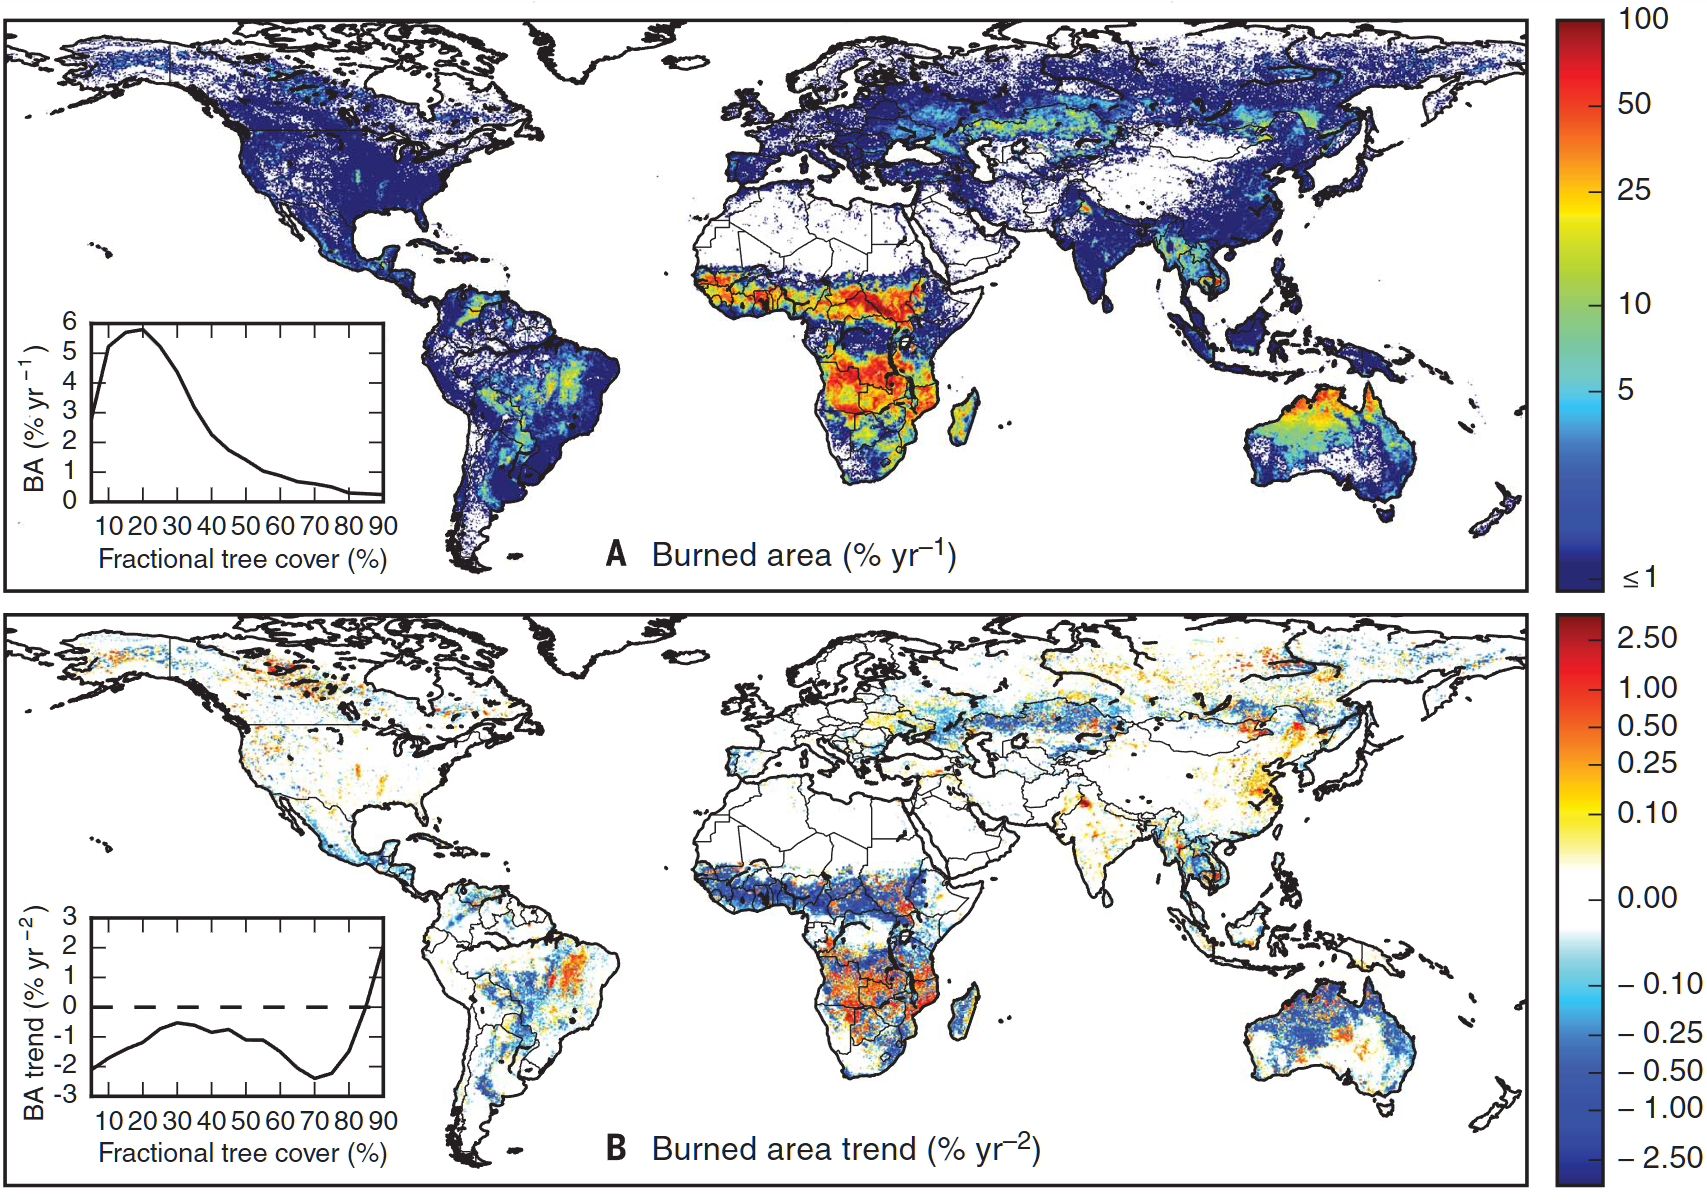
\includegraphics[width=1\linewidth]{images/map_BA_global_decrease_1998_2015.png}
%     \caption{\small{Satellite observations show a declining trend in fire activity across the world’s tropical and temperate grassland ecosystems and land-use
% frontiers in the Americas and Southeast Asia. (A) mean annual burned area and (B) trends in burned area (GFED4s, 1998 through 2015). Line plots (inset)
% indicate global burned area and trend distributions by fractional tree cover}}
%     \label{fig:map_BA_global_decrease_1998_2015}
% \end{figure}



% Explan correlations

% \begin{figure}[H]
%     \centering
%     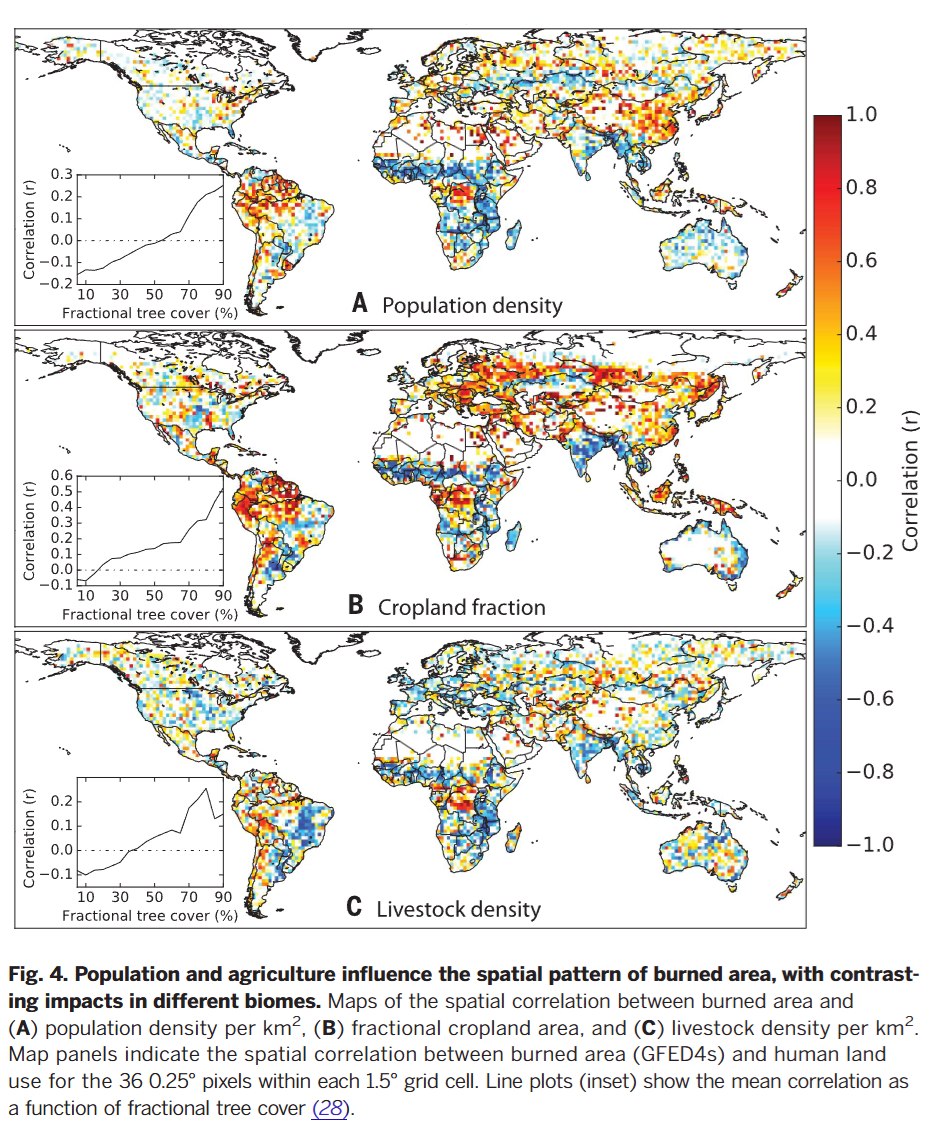
\includegraphics[width=1\linewidth]{images/map_BA_correlation_population_cropland_livestock.png}
%     \caption{Enter Caption}
%     \label{fig:map_BA_correlation_population_trends}
% \end{figure}
% \subsubsection{Increase in Regional Burned Area}

% Although global BA has declined since the 2000s, multiple studies report regional increases in burned areas in different types of ecosystems. Fig \ref{fig:map_BA_global_decrease_1998_2015} -B demonstrates the regions where the burned area trend is still increasing. The design of the satellite constellation shall have as secondary Regions of Interest (ROIs) the ecoregions with frequent incident wildfires. This subsection's goal is to indicate what these potential ROIs are, give details of recent BA activity, and provide some correlations that is connected with the fire activity. 

% Andela et al. (2017) found that, despite a ~24\% global BA decline (1998–2015), areas of significant BA increase were widespread across Eurasia’s closed-canopy forests (boreal and temperate), even as savanna/grassland BA—the dominant global contributor—contracted with cropland expansion, grazing, and fuel fragmentation. 

% Jones et al. (2001–2019) report rising BA in several forest ecoregions—e.g., Pacific U.S. forests (~+49\%), Pacific Canada (~+63\%), and East Siberian boreal forests (~+93\%)—noting that short records and high interannual variability make some trends statistically non-significant at the grid/ecoregion scale. 

% Extending the satellite record, GFED5 (1997–2020) shows positive BA trends across many high-northern boreal ecosystems (e.g., Siberia and the Russian Far East), consistent with warming-driven fuel aridity and longer fire seasons in closed-canopy needleleaf forests. 

% Complementary evidence based on forest loss attributed to fire (2001–2019) indicates a global increase in fire-related forest loss, with strongest contributions from boreal Eurasia, and additional signals in humid/tropical and temperate forests, underscoring that forest biomes (rather than savannas) are driving the emergent increases. 

% Looking over longer baselines, circumboreal syntheses show ~50\% higher BA from the 1980s to the 2010s, with significant increases over substantial closed-canopy areas, reconciling the global decline (savanna-driven) with rising forest fire activity at higher latitudes.

% \begin{figure}[H]
%     \centering
%     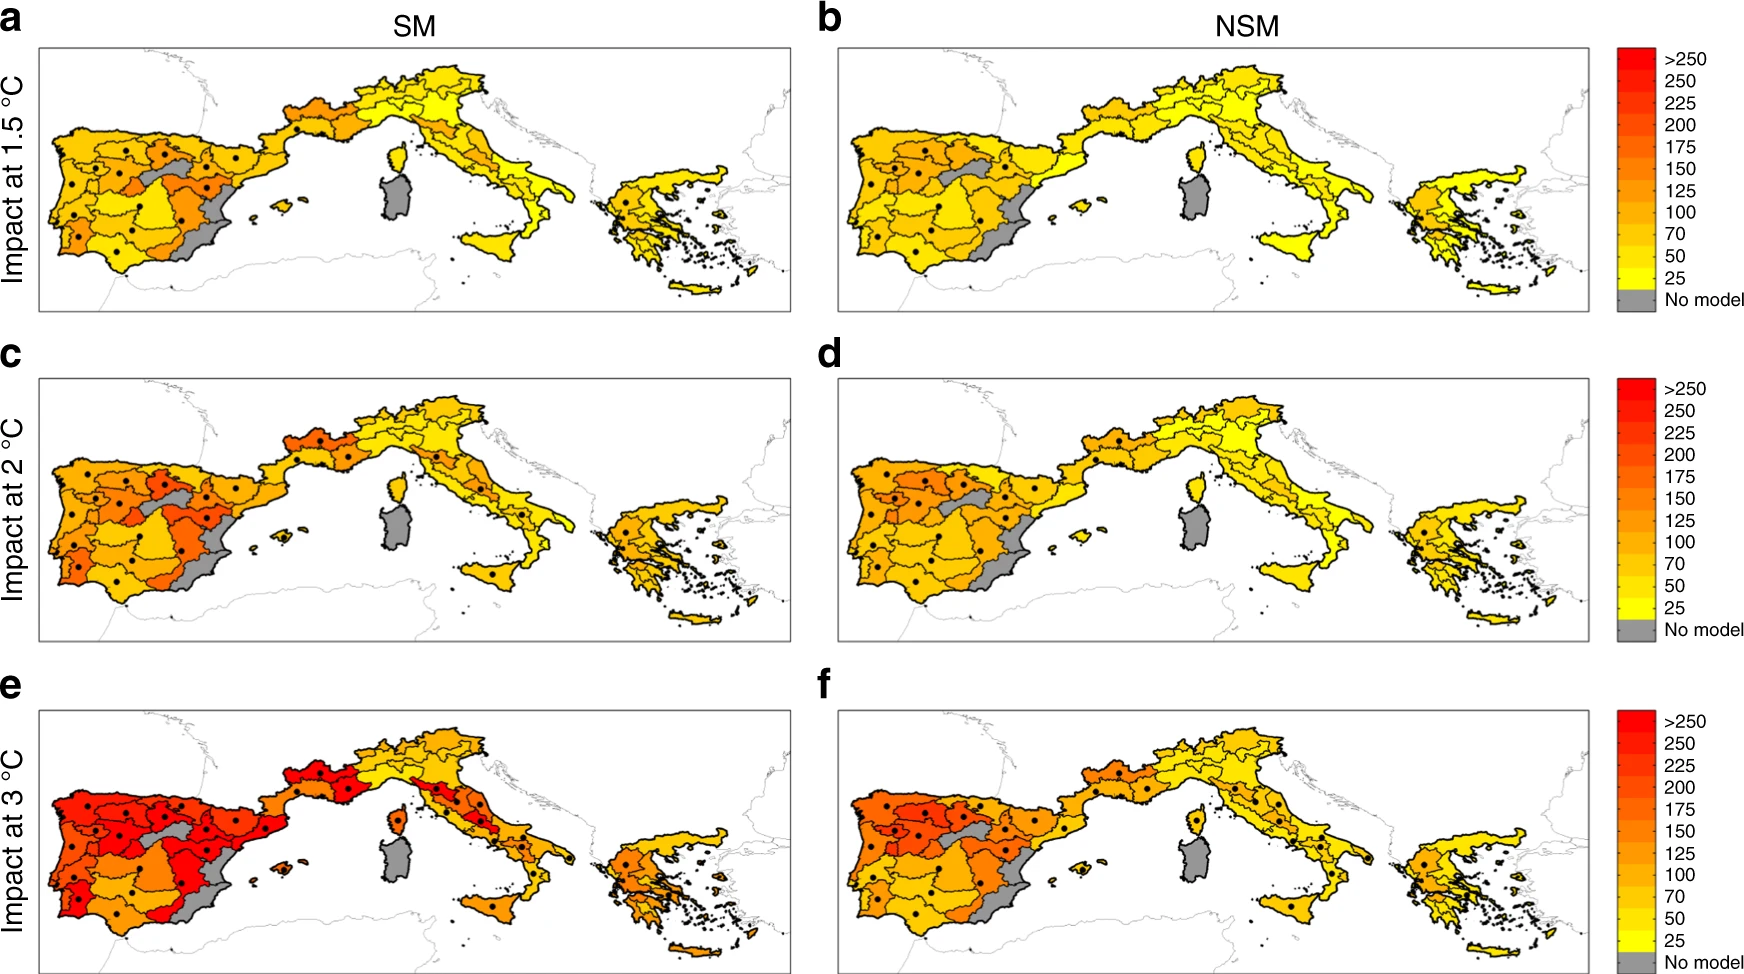
\includegraphics[width=1\linewidth]{images/mediterranean_fire_increase.png}
%     \caption{Ensemble mean burned area changes. Burned area changes (\%) for a the +1.5°C case with the stationary model SM (i.e., using Eq. 3), (b) the +1.5°C case with non-stationary model NSM (i.e., NSM). using Eq. (4), (c) the +2°C case with SM, (d) the +2°C case with NSM, (e) the +3°C case with SM, and f the +3°C case with NSM. Dots indicate areas where at least 50\% of the simulations (1000 bootstrap replications × the ensemble of RCMs) show a statistically significant change and more than 66\% agree on the direction of the change. Coloured areas (without dots) indicate that changes are small compared to natural variations, and white regions (if any) indicate that no agreement between the simulations is found}
%     \label{fig:mediterranean_fire_area}
% \end{figure}


% \subsection{Burned Area Trends Vs Correlations}






% \subsubsection{Rise of Forest Burned Area}

% IPCC-assessed projections indicate Mediterranean burned area could increase by \(\sim\)40–54\% at 1.5\(^{\circ}\)C, 62–87\% at 2\(^{\circ}\)C, and 96–187\% at 3\(^{\circ}\)C, with compound hot–dry extremes and drought driving large-fire risk\cite{turco_exacerbated_2018}.\footnote{\textit{Side note—Mediterranean risk:} Tenfold increases in the probability of catastrophic fire years are possible in parts of southern Europe under moderate CMIP6 scenarios \cite{elgarroussi_europe_2024}, and repeated fires can shift Mediterranean forests toward shrublands; paleorecords show that crossing precipitation thresholds ($\approx$40–45\% below interglacial levels) triggered abrupt forest–to–steppe transitions in the past, underscoring limited resilience under sustained aridification \cite{koutsodendris_atmospheric_2023,baudena_increased_2020}. The Mediterranean warms \(\sim\)20\% faster than the global average and WUI now covers \(\sim\)7.4\% of Europe, heightening exposure; recent EFFIS/JRC reports confirm that 2023 was among the worst EU wildfire years on record, dominated by the Mediterranean.} 

% The study done by Abatzoglou et al.\cite{abatzoglou_global_2019} also indicates the affected area is projected to enlarge under continued warming. In places where vegetation and ignitions are available, this translates into rising fire potential and heightened management challenges, which call for orbital sensors to assist in wildfire management \cite{abatzoglou_global_2019}.



% \section{Event cycles of wildfire --- Global \& Portuguese
% case}\label{22-event-cycles-of-wildfire-----global--portuguese-case}

% Show \textbf{global/biome monthly seasonality} (heatmaps or histograms)
% to characterize \emph{when} fires occur by regime; produce a neutral
% \textbf{seasonality atlas} of peak months across major pyro-regions.
% \textbf{Output:} a global reference calendar used later to benchmark
% Portugal and to define optional \textbf{secondary performance
% capability} tests for a Portugal-centric constellation in other regions'
% peak seasons.

% \begin{figure}
%     \centering
%     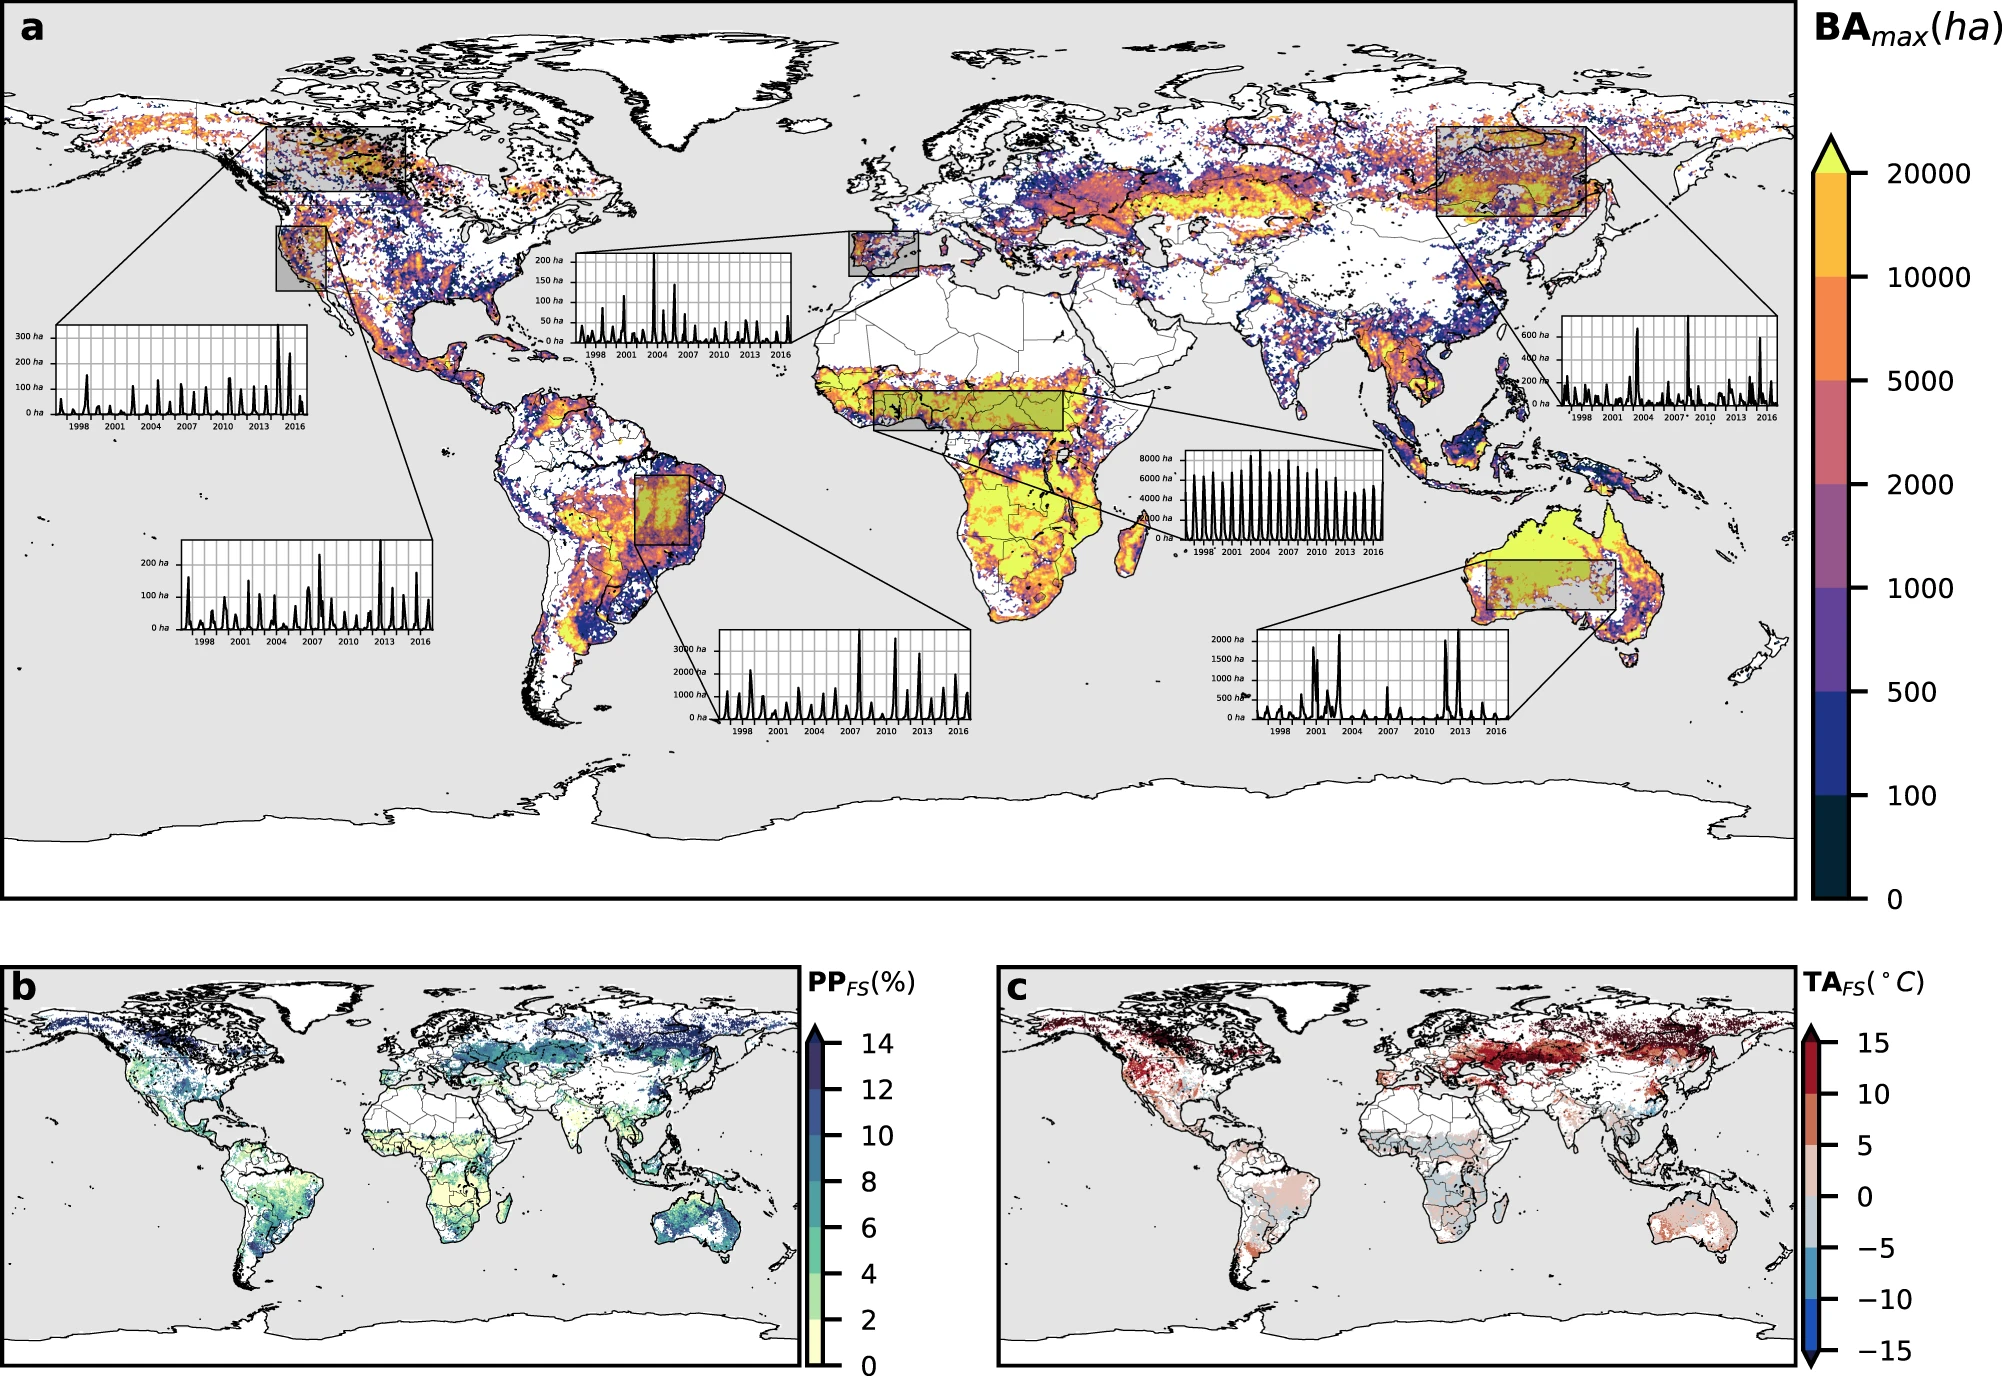
\includegraphics[width=1\linewidth]{images/BA_global_decade_fire_seasons.png}
%     \caption{1996–2016 maximum annual burned area (BAmax) and monthly burned area time series for selected regions. b Average monthly precipitation percentage from the annual total for the fire season (PPFS). c Average monthly temperature anomaly from the annual mean for the fire season (TAFS) https://www.nature.com/articles/s41467-022-28835-2/figures/1.}
%     \label{fig:BA_global_decade_fire_seasons}
% \end{figure}

%--------------------

This chapter establishes the observational study domains that define where and when the satellite constellation must observe. It begins by formalising the mission environment as a four-dimensional manifold connecting the inertial and Earth-fixed reference frames, and then defines two complementary study domains: the \textit{Core Study Domain} ($\mathcal{D}_{core}$), spatially bounded by mainland Portugal and temporally aligned with its fire season, and the \textit{Global Study Domain} ($\mathcal{D}_{global}$), which extends the analysis to all fire-prone regions classified by climate regime and fire frequency. The chapter concludes by introducing the FIRMS geostationary active-fire dataset as the high-cadence empirical reference for constellation verification, and by consolidating the derived requirements (R9--R25) that constrain the mission simulation.

\section{Observational Study Domains} \label{sec:obs_domains}

Depending on the dynamic interactions among biomass, climate, and human activity, each region of interest observed by the satellite could exhibit a characterizable fire intensity over a temporal pattern; in other words, each region of interest could have a specific fire season. With this in mind, the satellite constellation mission modeled in this work shall have as a requirement an observational temporal window synchronized with these fire season periods. Therefore, the spacecraft architecture shall be analyzed against\textit{ Fire-Prone Regions (FPR)}, or piroregions, here defined as the \textit{Core Study Domain ($\mathcal{D}_{core}$)} and the \textit{Generalized Study Domain ($\mathcal{D}_{general}$)}. Both of these objects are composed of subsets of \textit{Regions of Interest (ROI)} which are defined in a spatial $\mathcal{R}$ and temporal $\mathcal{T}$ coordinate domains. Therefore, each ROI can contain flammable biomass that may exhibit distinct fire dynamics over time, leading to a temporal spread of \textit{Fire Activity (FA)} in these domains. 

\subsubsection{Formal Definition of Study Domains}\label{sec:formal_def_domains}

To ensure the satellite constellation meets precise operational requirements, we define the mission environment as a four-dimensional manifold $\mathcal{M}$ (Space-Time). Since the satellite orbit is governed by orbital mechanics while the observation targets are subject to planetary dynamic motion, we must rigorously define the relationship between the inertial and rotating frames.

We establish the base reference frame of $\mathcal{M}$ as the \textbf{Earth Mean Equator and Equinox of J2000 (EME2000)}, hereafter denoted as the Inertial Frame $\mathcal{F}_{J2000}$ (corresponding to the IJK system in Fig. \ref{fig:vallado_ijk_frame}). However, the regions of interest for the constellation are fixed to the rotating Earth. Therefore, we define the boundaries of the study domains relative to the \textbf{World Geodesic System 84 (WGS84)}, which has an Earth-Centered Earth-Fixed (ECEF) frame, hereafter denoted as the Earth Frame $\mathcal{F}_{\oplus}$, \inlineReq{R9}.
\begin{figure}[H]
    \centering
    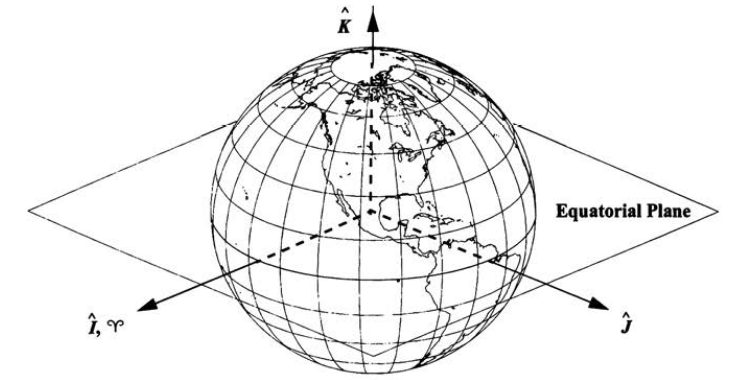
\includegraphics[width=0.65\linewidth]{images/Geocentric_Equatorial_System_(IJK)_F_earth.png}
    \caption{\footnotesize{The Geocentric Equatorial Coordinate System (IJK) as defined by Vallado \cite{mcclain2001fundamentals}. The frame is defined by Earth's origin, the equatorial plane, and the vector $\hat{I}$ pointing toward the Vernal Equinox ($\Upsilon$). In this thesis, the IJF frame system represents the Inertial Frame $\mathcal{F}_{J2000}$ used for orbit propagation. It is distinct from the rotating Earth Frame $\mathcal{F}_{\oplus}$ (ECEF), which holds the study Domain $\mathcal{D}$ that rotates with the Earth.}}
    \label{fig:vallado_ijk_frame}
\end{figure}
Formally, the universal manifold $\mathcal{M}$ is defined as the Cartesian product of spatial and temporal domains, mathematically expressed as:

\begin{equation}
    \mathcal{M} = \mathbb{E}^3 \times \mathcal{T} \cong \{ (P, t) \}
    \label{eq:manifold}
\end{equation}

Here, $\mathbb{E}^3$ denotes the 3-dimensional spatial Euclidean Space, while $\mathcal{T}$ represents the absolute time continuum expressed in Coordinated Universal Time (UTC) . The relation $\mathcal{T} \cong \mathbb{R}$ establishes the structure-preserving mapping, or isomorphism, between physical time and the real number line, ordered by the epoch $t$. Consequently, any unique event in the manifold is represented by the pair $(P, t)$, where $P \in \mathbb{E}^3$ is a spatial point and $t \in \mathcal{T}$ is a temporal moment.

To enable orbital analysis within this manifold $\mathcal{M}$ , we define an origin $O$ at the Earth's Center of Mass. This definition permits the mapping of any spatial point $P$ to a position vector $\mathbf{r}$ in the inertial frame $\mathcal{F}_{J2000}$ via the transformation $\mathbf{r} = P - O$.

A Study Domain $\mathcal{D} \subset \mathcal{M}$ is defined as the subset of inertial points occupied by a specific geographic region of interest $ROI_{\text{W84}}$ during a specific temporal fire season window $\mathcal{T}_{fire}$. Mathematically, this domain is expressed as:
\begin{equation}
    \mathcal{D} = \{ (\mathbf{r}_{J2000}, t) \in \mathcal{M} \mid \mathbf{r}_{J2000} = \mathbf{T}_{\oplus \to J2000}(t) \cdot \mathbf{r}_{\oplus}(\phi, \lambda, h), \ t \in \mathcal{T}_{fire} \}
\end{equation}
In this formulation  $\mathbf{r}_{\oplus}(\phi, \lambda, h)$ denotes the position vector in the Earth Frame $\mathcal{F}_{\oplus}$, derived from the geodetic coordinates of latitude $\phi$, longitude $\lambda$, and altitude $h$. The target observation fire season is represented by $\mathcal{T}_{fire} = [t_{start}, t_{end}]$ in UTC. $\mathbf{T}_{\oplus \to J2000}(t)$ is the time-dependent coordinate transformation. This operator accounts for Earth’s rotation, precession, and nutation, projecting the fixed ground coordinates from $\mathcal{F}_{\oplus}$ into the inertial frame $\mathcal{F}_{J2000}$.  

This process of coordinate transfers of study domain $\mathcal{D}$ rotating on Earth's frame to an inertial frame allows calculations connecting $\mathcal{D}$ with the satellite propagation, making possible knowledge such coverage time, revisits, communication links, satellite imagery retrieval from datasets, etc.

Using this study domain formalism, we define the two primary objects of this study:
\begin{itemize}
    \item \textbf{Core Study Domain ($\mathcal{D}_{core}$)}: The subset of $\mathcal{M}$ constrained by the geographical boundaries of Mainland Portugal and the temporal bounds of its fire season\inlineReq{R10}.
    \item \textbf{Global Study Domain ($\mathcal{D}_{global}$)}: The subset of  $\mathcal{M}$  containing Earth's fire-prone regions each with a specific temporal fire activity \inlineReq{R11}.
\end{itemize}

\subsection{Core Study Domain}

This section details the properties of $\mathcal{D}_{core}$, establishing its spatial region elements $\mathcal{R}_{core}$ and core temporal boundaries $\mathcal{T}_{core}$ for the definition of the mission over mainland Portugal. Formally, the domain is defined as the Cartesian product of these spatial and temporal sets:
\begin{equation}
    \mathcal{D}_{core} = \mathcal{R}_{core} \times \mathcal{T}_{core} \subset \mathcal{M}
\end{equation}
This definition is useful for analysis, such as observation events that require the satellite state vector or field of view to coincide with points $p \in \mathcal{R}_{core}$ at a time $t \in \mathcal{T}_{core}$. 

\subsubsection{Core Spatial Elements}

The spatial component $R_{core}$ is composed of a set of geometrical objects defined on the reference ellipsoid of the WGS84 system. We categorize these objects into two topological types:

\begin{enumerate}
    \item \textbf{Point Target (P):} Defined as a single vertex coordinate $P(\phi, \lambda, h)$, representing a point with zero-dimensional location of interest (e.g., a ground target, specific ground station, or a city location).

    \item \textbf{Region Target ($\mathcal{R}$):} Defined as the union of $M$ distinct surface patches $S_j$. Mathematically, the region target is a multi-polygon defining a compact region $\mathcal{R} = \bigcup_{j=1}^{M} S_j$. Each patch $S_j$ is a surface bounded by a closed geodesic polygon. The boundary of such a polygon $S_j$, denoted as $\partial S_j$, is a piecewise geodesic curve consisting of connected geodesic segments defined by an ordered set of $N_j$ vertices $\{P_{i}\}_{i=1}^{N_j} = \{P_{1}, P_{2}, ..., P_{N_{j}}\}$, where the boundary is closed by the segment $P_{N_{j}}$ to $P_{1}$.
\end{enumerate}

% \begin{figure}[ht]
%   \centering
%   \fbox{%
%     \begin{minipage}[c][1cm][c]{0.9\linewidth}
%       \centering \textit{[Figure placeholder: Diagram: Point Target P vs. Region Target $\mathcal{R}$ defined by Geodesic Boundary]}
%     \end{minipage}%
%   }
%   \caption{Topological definition of Point and Region targets on the WGS84 Ellipsoid.}
%   \label{fig:drawing_core_spatial_elements}
% \end{figure}

\subparagraph{Application to Mainland Portugal ($\mathcal{R}_{pt}$)}\hspace{0pt}

Applying these definitions, the spatial region of mainland Portugal is modeled as a Region Target $\mathcal{R}_{pt}, \inlineReq{R12}$. 
Its boundary, $\partial \mathcal{R}_{pt}$, is established using standard geospatial vector data formats, specifically ESRI Shapefiles (.shp) or GeoJSON. \footnote{These files encode the set of vertex coordinates $\{P_{i}\}_{i=1}^{N_j}$ in the Coordinate Reference System (CRS) EPSG:4326 (WGS84 Latitude/Longitude). For the computational simulation, these geometries are processed using standard Python geospatial modules, such as \texttt{geopandas} for data management and \texttt{shapely} for geometric operations (e.g., point-in-polygon verification, coverage maps).}
At figure \ref{fig:map_D_core_elements}, $\mathcal{R}_{pt}$ can be visualized.


\subparagraph{Application to points inside Portugal 
($\mathcal{P}_{pt}$)}\hspace{0pt}
\label{sec_pt_space_domain}
 
It is interesting to define point targets $P_i$ within Portugal's $\mathcal{R}_{pt}$ boundaries to verify the local performance of the satellite constellation, such as the revisit time over a city or fire-prone location. 
To decide which points to choose, we perform the following verification. One can analyze studies of burned area
%as figuras estão com link quebrados
%(Fig \ref{fig:map_BA_global_decrease_1998_2015}, Fig \ref{fig:BA_global_decade_fire_seasons}) 
and fire activity (Fig.\ref{fig:fire_season_types}  to  Fig. \ref{fig:fire_season_start2_end2}). The combination of this kind of multivariate study can lead to the production of a global map of fire-climate classes stratified by the intensity of each fire-prone region, as done by Senande-Rivera et al., reproduced here in Fig  \ref{fig:fire_prone_global_now_future}-b \cite{senande-rivera_spatial_2022}. 

As seen in Rivera's work, Portugal and most of the Iberian Peninsula have a fire-climate class defined as Temperate-dry hot season (Te-dhs), with recurrent (r) fire-prone regions quantified by more than seven intense fires per decade. More specifically, this zone is defined as Te-dhs-r (Temperate-dry hot season-recurrent, or the temperate belt latitude  ($\phi \approx \pm\,[30^{\circ}$--$45^{\circ}]$)). Because this peninsular area exhibits almost homogeneous fire dynamics, the best strategy to achieve optimal constellation coverage is to select a point target centralized in Portugal. As we wish this point to be revisited often by the satellite constellation, this central point is named $P_{revisit}$.
Therefore, this work selects Coimbra as the main target to revisit inside the core study domain because it is the largest city, approximately in the center of Portugal, and surrounded by fire-prone regions \inlineReq{R13}. 
\begin{equation}
    P_{revisit} = P_{Coimbra}
\end{equation}


To verify the satellite constellation performance in other relevant Portuguese i points $\mathcal{P}_{pt,i}(\phi, \lambda, h)$, the table \ref{tab:pt_coords} with geographical references will be used during the simulation\inlineReq{R14}. This points are visualized in the map \ref{fig:map_D_core_elements}.

\begin{table}[ht]
\centering
\caption{Point target coordinates $\mathcal{P}_{pt,i}(\phi, \lambda, h)$ of selected regions of interest inside the Portugal mainland region target $\mathcal{R}_{pt}$ which is contained in the core study domain $\mathcal{D}_{core}$. (WGS84).}
\label{tab:pt_coords}

\begin{tabular}{lrrr}
\toprule
Location ($P_{pt,i}$) & Latitude $\phi$ [$^\circ$] & Longitude $\lambda$ [$^\circ$] & Altitude $h$ [m]\\
\midrule
Coimbra (Reference) & 40.20329 & -8.41389 & 90 \\
Leiria              & 39.75000 & -8.80000  & 80 \\
Fundão              & 40.13300 & -7.50000  & 500 \\
Castelo Branco      & 39.81700 & -7.50000  & 320 \\
Serra da Estrela    & 40.32187 & -7.61297  & 1993 \\
Porto               & 41.15000 & -8.61083  & 100 \\
Lisboa              & 38.72528 & -9.15000  & 77 \\
Faro                & 37.01611 & -7.93500  & 10 \\
\bottomrule
\end{tabular}
\end{table}

\begin{figure}[H]
    \centering
    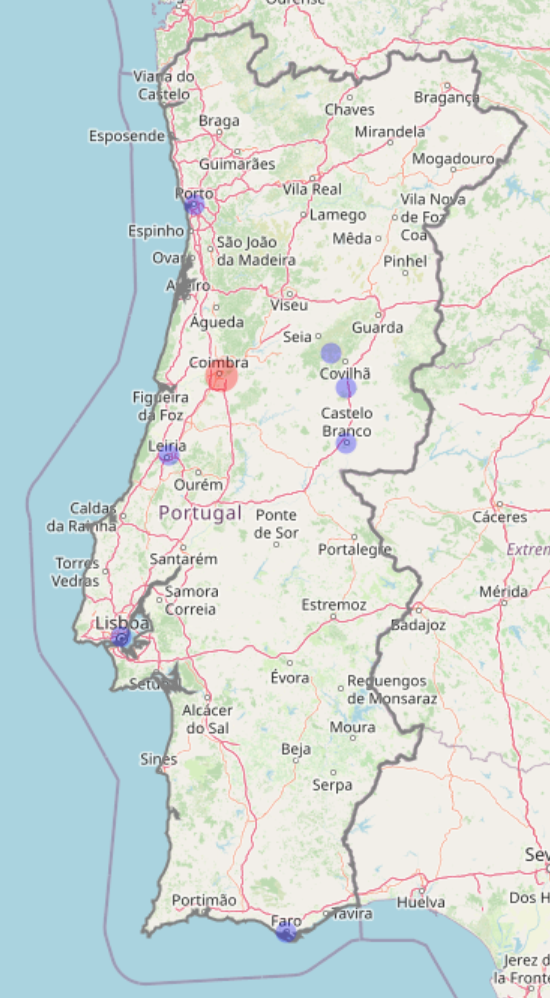
\includegraphics[width=0.3\linewidth]{images/map_D_core_elements2.png}
    \caption{\footnotesize{Core study domain $\mathcal{D}_{core}$ defined by Portugal region $\mathcal{R}_{pt}$ and the inner target points $\mathcal{P}_{pt,i}$.  }}
    \label{fig:map_D_core_elements}
\end{figure}


\subsubsection{Core Temporal Boundaries}

With the core spatial region $\mathcal{R}_{core}$ established for Mainland Portugal, $\mathcal{R}_{core} \equiv \mathcal{R}_{pt}$, the core study domain now requires a observational window here, represented as a temporal set $\mathcal{T}_{core}\subset\mathcal{T}$ describing the  fire season expected to occur and for which the satellite constellation shall have the performance assessed.

 We establish the full year of 2024 as the simulation core temporal  \inlineReq{R15}. Formally, $\mathcal{T}_{core}$ is defined as the continuous interval:
\begin{equation}
    \mathcal{T}_{core} = [t_{start_{2024}}, t_{end_{2024}}] \subset \mathcal{T}
\end{equation}
Where $t_{start_{2024}}$ corresponds to 2024-01-01 00:00:00 UTC and $t_{end_{2024}}$ to 2024-12-31 23:59:59 UTC.

\subparagraph{Portugal season markers}\hspace{0pt}

A detailed global study of fire season types was done by Zhang et al \cite{zhang_global_2025}. They used satellite-based Moderate Resolution Imaging Spectroradiometer (MODIS) burned area records (2001–2022) to classify global fire season types by the number of peaks, or modals, within a year. Globally, three fire season categories were identified: unimodal (31.25\%), bimodal (52.07\%), and random (16.69\%), as shown in Fig. \ref{fig:fire_season_types} and Fig. \ref{fig:map_global_fire_season_types}. Unimodal fire seasons occur mainly in boreal and tropical zones and last about 2.7 months, whereas temperate ecosystems typically have longer, bimodal fire seasons (~3 months) with two peaks per year. Portugal is classified as a temperate ecosystem with a bimodal fire season type.

To define the core study fire Season in Portugal, one can follow the definition of fire season presented in Fig. \ref{fig:fire_season_types}, where the bimodal general annual fire activity curve defines the day of year of the fire season onset $t_{\text{start}}$, two fire activity peaks instants $t_{\text{peak},1}$ and $t_{\text{peak},2}$,  finalizing with $t_{\text{end}}$. 

A survey of the fire-season marker maps (Fig.~\ref{fig:fire_season_start_end}--Fig.~\ref{fig:fire_season_start2_end2}) indicates moderate spatial heterogeneity across Portugal. For mission-level analysis, we therefore adopt indicative bounds that conservatively cover the earliest onset, the two dominant August peaks, and the late-season decay into February. The resulting marker set for a season year  is summarized in Table~\ref{tab:pt_fire_season_bounds}.

\subparagraph{Critical observational reference for the constellation}\hspace{0pt}

Portugal's fire season starts in March, with increasing fire activity peaking in summer. This is the critical observation period for the constellation, which has two main intense peaks in the first week of August and around the third week. The constellation shall have the best coverage in this month, with August 18 as the main fire peak reference \inlineReq{R16}. 
\begin{equation}
    t_{\text{peak fire ref}} = \text{ August 18th }
    \label{eq:peak_fire_ref_day}
\end{equation}
After this period of faster pyrodynamics, the season extends with decreasing intensity until fading in February of the next year. 


\begin{table}[ht]
\centering
\caption{\footnotesize{Definition of the Core Temporal Boundaries $\mathcal{T}_{core}$ for Portugal, detailing the two phenomenological sub-periods and peaks based on Day-of-Year (DOY).}}
\label{tab:pt_fire_season_bounds}
\renewcommand{\arraystretch}{1.2}
\begin{tabular}{lll p{5.5cm}}
\toprule
\textbf{Season Marker} & \textbf{Symbol} & \textbf{Date: (DOY)}& \textbf{Interpretation} \\
\midrule
Start fire subperiod 1 
& $t_{start,1}$
& Mar 11 ($\sim 70$)
& Earliest onset of fire activity. \\

1th peak& $t_{peak,1}$
& Aug 08 ($\sim 220$)
& First local peak of the bimodal cycle. \\

End fire subperiod 1 
& $t_{end,1}$
& Aug 13 ($\sim 225$)
& Transition to the core intensity period. \\

\midrule

Start fire subperiod 2 
& $t_{start,2}$
& Aug 13 ($\sim 225$)
& Onset of the critical design period. \\

2th peak& $\mathbf{t_{peak,2}}$
& \textbf{Aug 18 ($\sim 230$)}
& \textbf{Strongest seasonal peak. Critical design point.} \\

End fire subperiod 2 
& $t_{end,2}$
& Feb 09 ($\sim 40^*$)
& Latest tail end (referring to the subsequent year). \\
\bottomrule
\end{tabular}
\end{table}


\begin{figure}[H]
    \centering
    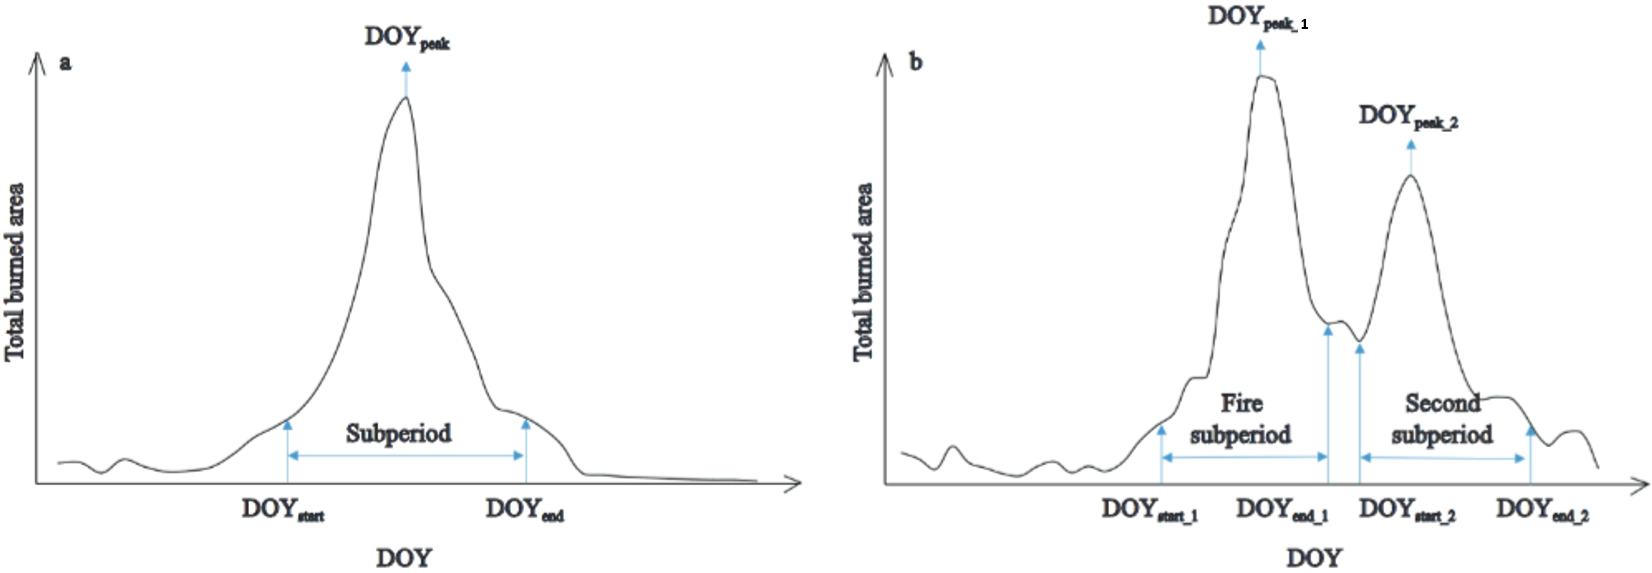
\includegraphics[width=1\linewidth]{images/fire_season_types.png}
    \caption{\footnotesize{The schematic diagram of unimodal (a) and bimodal (b) fire season types. The fire season starts on the day of year $\mathrm{DOY}_{\text{start}}$, it has peaks $\mathrm{DOY}_{\text{peak}}$, and ends on $\mathrm{DOY}_{\text{end}}$. \protect\footnotemark}}
    \label{fig:fire_season_types}
\end{figure}


\footnotetext{\label{fn:Zhang2025}Adapted from Zhang \emph{et al.} (2025)~\cite{zhang_global_2025}.}


\begin{figure}[H]
    \centering
    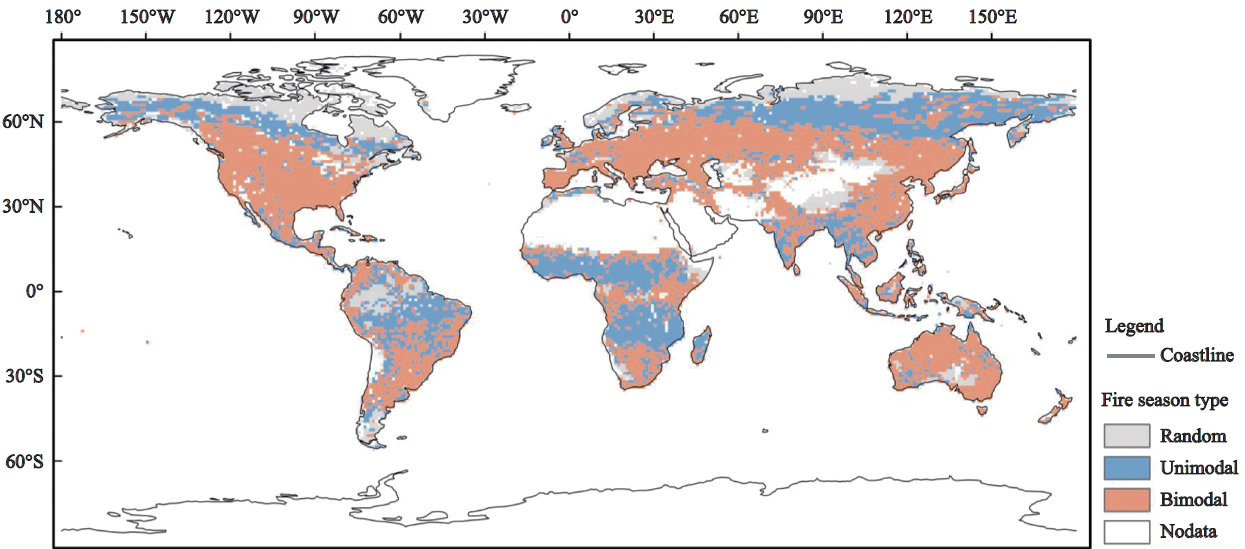
\includegraphics[width=0.65\linewidth]{images/map_global_fire_season_types.png}
    \caption{\footnotesize{Global distributions of fire season types from 2001 to 2022.  \textsuperscript{\ref{fn:Zhang2025}}}}
    \label{fig:map_global_fire_season_types}
\end{figure}

% \begin{figure}[H]
%     \centering
%     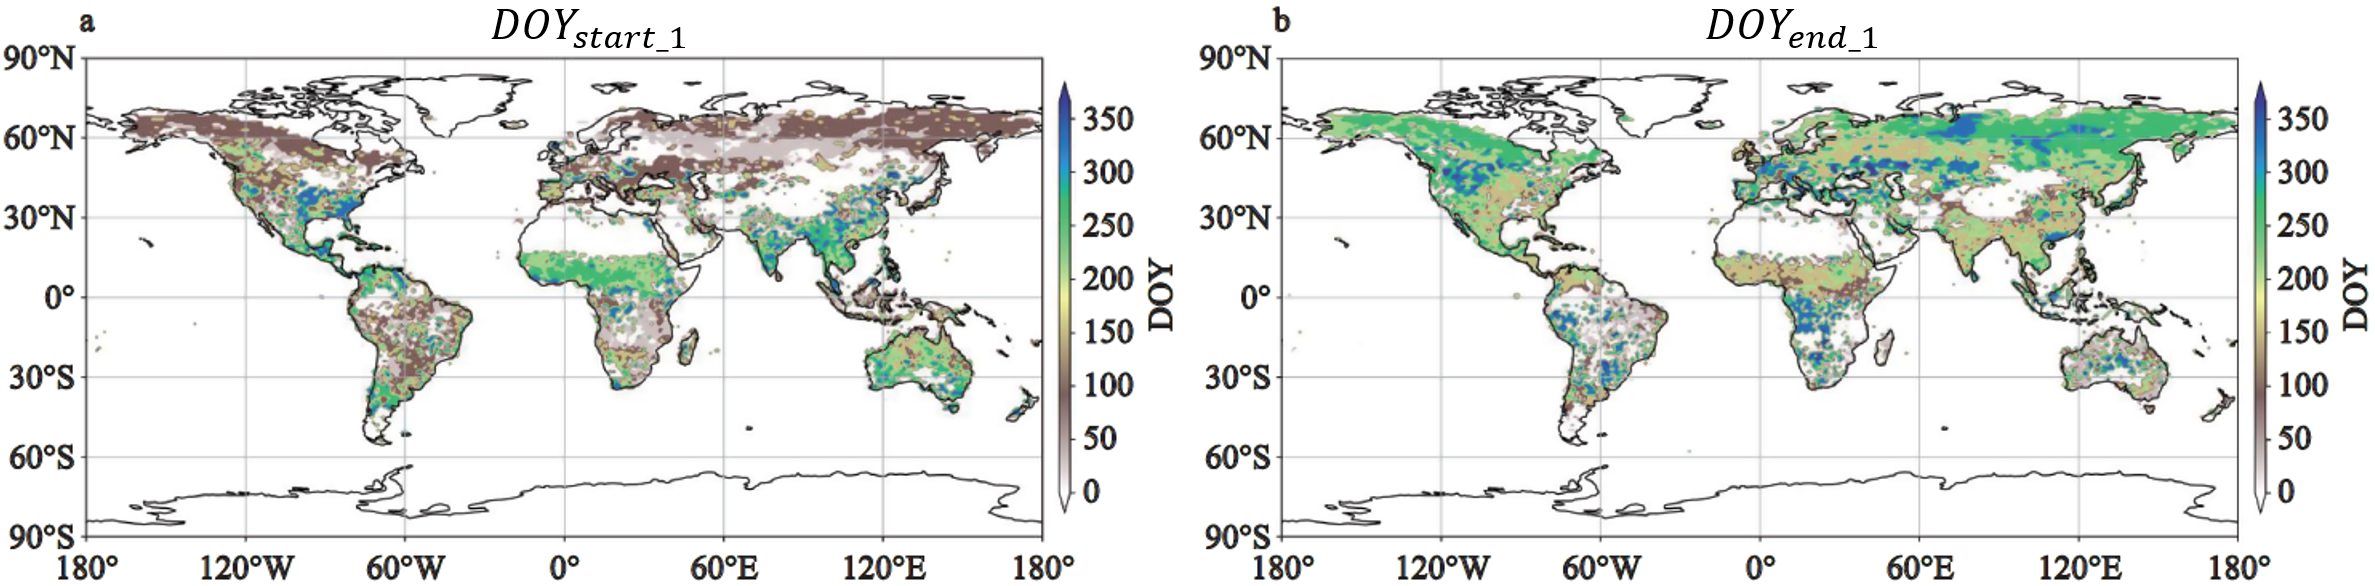
\includegraphics[width=0.9\linewidth]{images/fire_season_start1_end1.png}
%     \caption{\footnotesize{Global distributions of the fire season first subperiod (see Fig. \ref{fig:fire_season_types})  start day of year $\mathrm{DOY}_{\text{start 1}}$  (a) and end $\mathrm{DOY}_{\text{end 1}}$ (b).  \textsuperscript{\ref{fn:Zhang2025}}}}
%     \label{fig:fire_season_start_end}
% \end{figure}

% \begin{figure}[H]
%     \centering
%     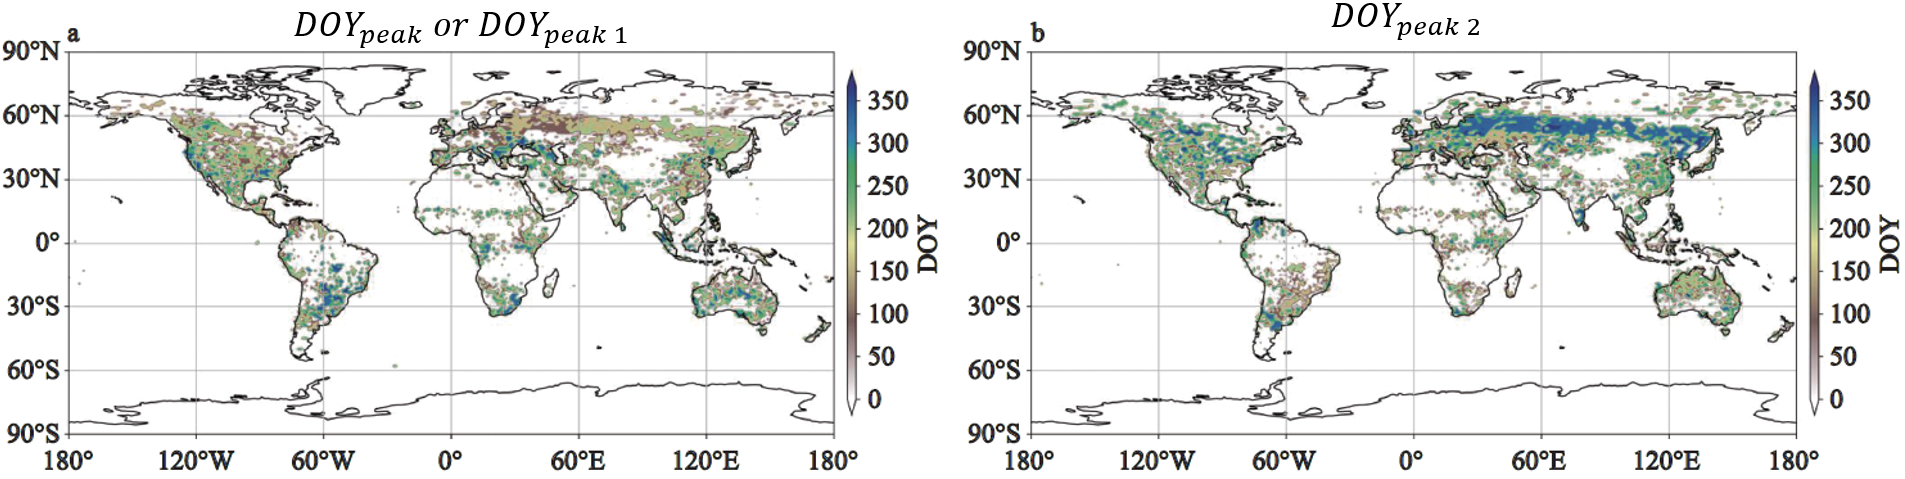
\includegraphics[width=0.9\linewidth]{images/fire_season_peaks.png}
%     \caption{\footnotesize{Global distributions of the peak start day of year $\mathrm{DOY}_{\text{peak} 1}$ in the first subperiod (a) and second subperiod $\mathrm{DOY}_{\text{peak}  2}$(b) of fire season from 2001 to 2022. See Fig. \ref{fig:fire_season_types} about subperiods.  \textsuperscript{\ref{fn:Zhang2025}}}}
%     \label{fig:fire_season_peaks}
% \end{figure}

% \begin{figure}[H]
%     \centering
%     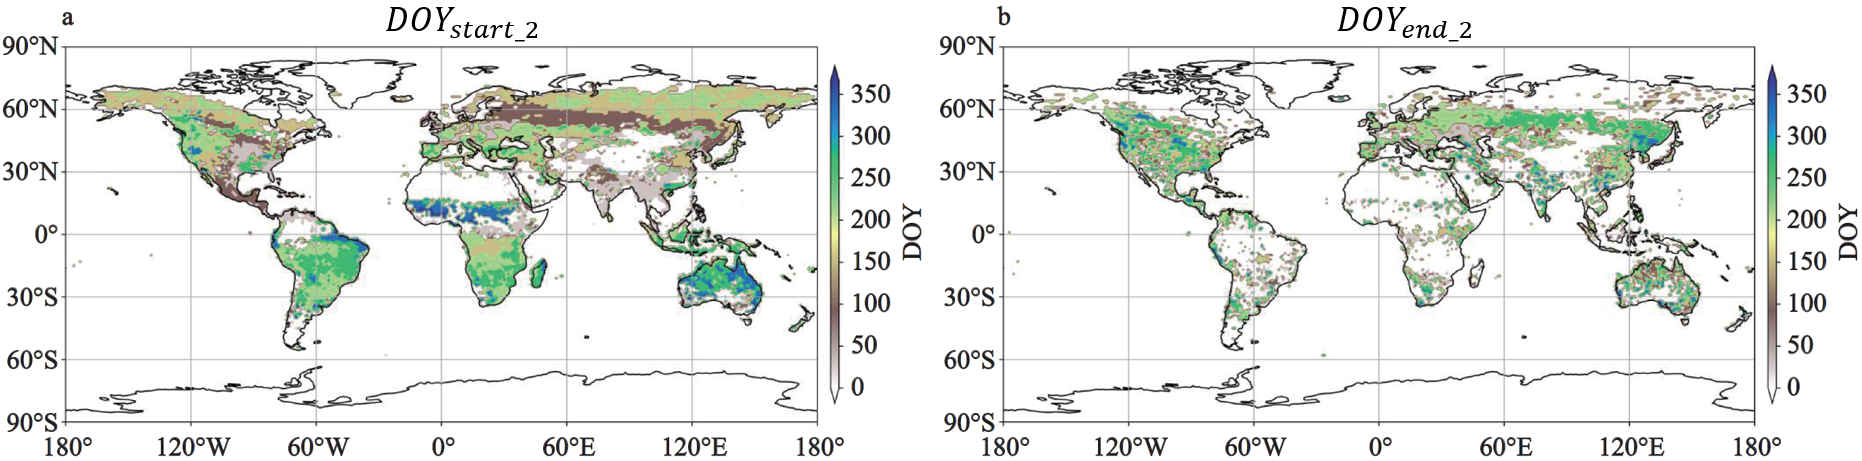
\includegraphics[width=0.9\linewidth]{images/fire_season_start2_end2.png}
%     \caption{\footnotesize{Global distributions of the fire season second subperiod (see Fig. \ref{fig:fire_season_types})  start day of year $\mathrm{DOY}_{\text{start 2}}$  (a) and end $\mathrm{DOY}_{\text{end 2}}$ (b).  \textsuperscript{\ref{fn:Zhang2025}}}}
%     \label{fig:fire_season_start2_end2}
% \end{figure}

% \begin{figure}[ht]
%   \centering
%   \fbox{%
%     \begin{minipage}[c][1cm][c]{0.9\linewidth}
%       \centering \textit{Figure placeholder}
%     \end{minipage}%
%   }
%   \caption{TODO: Add histogram of active fire in the GOEs dataset for portugal and identify the peaks, connect it to the global domain if makes sense}
%   \label{fig:placeholder_text}
% \end{figure}


\subsection{Generalized Study Domain}
\label{sec:generalized_study_domain}

This section details the properties of the Global Study Domain $\mathcal{D}_{global}$, establishing its spatial region elements $\mathcal{R}_{global}$ and temporal boundaries $\mathcal{T}_{global}$. Formally, the domain is defined as the Cartesian product of these sets:
\begin{equation}
    \mathcal{D}_{global} = \mathcal{R}_{global} \times \mathcal{T}_{global} \subset \mathcal{M}
\end{equation}

\subsubsection{Global Spatial Element}

To construct the global spatial definition, we extend the previous topological concepts of the Core Domain. However, unlike $\mathcal{R}_{core}$, which is bounded by static geopolitical borders (Mainland Portugal), the global region $\mathcal{R}_{global}$ is defined by phenomenological boundaries, specifically, the probability of fire occurrence on different types of biomass and climate \inlineReq{R17}.

We designate this spatial object as the Earth's Fire-Prone Region Target\textbf{ $\mathcal{R}_{\oplus_{FPR}}$}. Mathematically, it is defined not as a single contiguous shape, but as the union of all disjoint surface patches $S_k$ on the planetary ellipsoid that have fire-prone characteristics:

\begin{equation}
    \mathcal{R}_{global} \equiv \mathcal{R}_{\oplus_{FPR}} = \bigcup_{k} S_k  \mid  \text{Class}(S_k) \in \mathcal{C}_{fire}
\end{equation}
Where $\mathcal{C}_{fire}$ represents the set of valid fire-prone regions classifications.

\subsubsection{Earth's Fire-Prone Regions Targets ($\mathcal{R}_{\oplus_{FPR}}$)} \hspace{0pt}
\label{sec:earths_frp_targets}

The boundaries of these surface $S_k$ are determined by the fire-climate classes derived from historical satellite data (as seen in Fig. \ref{fig:fire_prone_global_now_future}), methodology proposed by Senande-Rivera et al. \cite{senande-rivera_spatial_2022}. Consequently, $\mathcal{R}_{\oplus_{FPR}}$ acts as a spatial filter, restricting the mission analysis to relevant latitudes and ecosystems (e.g., Mediterranean, Savanna, Temperate) while excluding non-flammable regions (e.g., rainy regions, deserts, oceans, ice sheets). 

\begin{figure}
    \centering
    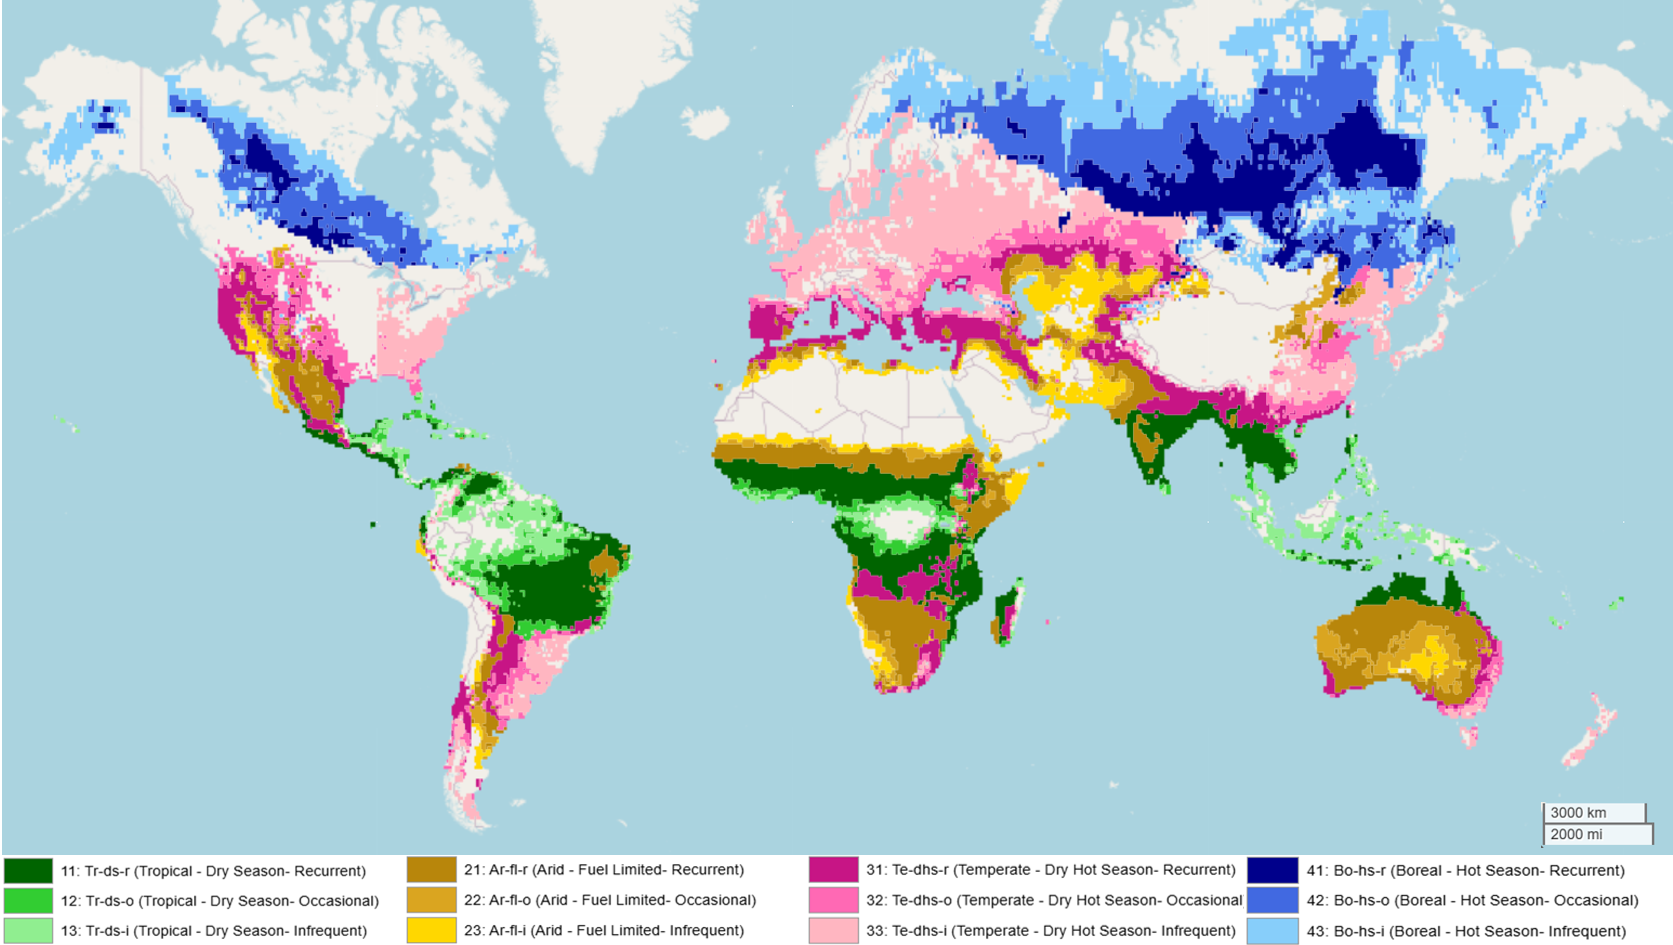
\includegraphics[width=1\linewidth]{images/map_earths_fireprone_region_targets.png}
    
    \caption{\footnotesize{\textbf{Spatial definition of the Earth's Fire-Prone Regions Target ($\mathcal{R}_{\oplus_{FPR}}$).} 
    The map visualizes the spatial element of the generalized study domain $\mathcal{R}_{global}$ as the union of all surface patches $S_k$ exhibiting valid fire-prone characteristics. Data is reconstructed from the \texttt{FC.nc} dataset provided by Senande-Rivera et al. \cite{senande-rivera_spatial_2022, senanderivera_fireclimate_2022}. The color coding corresponds to the specific fire-climate regimes $\alpha$ (e.g., \textit{Te-dhs-r}) defined in the taxonomy, stratified by climate (Tropical - Dry Season, Arid - Fuel Limited, Temperate - Dry Hot Season, Boreal - Hot Season), and fire frequency (Recurrent, Occasional, Infrequent). This spatial mask serves as the spatial operational filter for the constellation's global coverage analysis.}}
    
    \label{fig:map_earths_fire_prone_region_targets}
\end{figure}

\subparagraph{Classification Taxonomy}\hspace{0pt}

The classification assigns a descriptor to each region based on the nomenclature \texttt{[Climate]-[Type]-[Frequency]}.
First, regions are categorized into four primary climate regimes [Tropical, Arid, Temperate, Boreal] based on the Köppen–Geiger criteria. Then, specific fire thresholds are applied to identify the dominant phenomenological driver of fire activity (e.g., limited fuel vs. dry season). The intersection of these climatic and fire conditions defines the four primary classes presented bellow:

\begin{itemize}
    \item \textbf{Tr-ds (Tropical - Dry Season):} Regions driven by distinct dry seasons in tropical latitudes (e.g., Savannas).
    \item \textbf{Ar-fl (Arid - Fuel Limited):} Regions where fire activity is rare and constrained by available biomass rather than weather conditions.
    \item \textbf{Te-dhs (Temperate - Dry Hot Season):} Regions characterized by hot, dry summers (e.g., Mediterranean, Portugal). This is the primary analog to the Core Study Domain.
    \item \textbf{Bo-hs (Boreal - Hot Season):}High-latitude regions where fire activity is driven by seasonal heat waves and snow-melt timing.
\end{itemize}



\subparagraph{Frequency (Intensity)} \hspace{0pt}

Crucially for the satellite mission design of a fast wildfire constellation is the knoledge of the regions with higher frequency of fire. To assist on this goal, each climatic class is subdivided by intensity, defined by the number of \textit{Fire Prone Years (FPY)} per decade. This creates a hierarchy of observation priority:

\begin{enumerate}
    \item \textbf{Recurrent (r):} Regions with $> 7 FPY$/decade. These are high-priority targets requiring consistent monitoring if the coverage allows it depeding on the latitude.
    \item \textbf{Occasional (o):} Regions with $3 < FPY\text{/decade} \leq 7$.
    \item \textbf{Infrequent (i):} Regions with $0 < FPY\text{/decade} \leq 3$.
\end{enumerate}

\subparagraph{Operational Definition of the Global Target} \hspace{0pt}

For the purpose of this mission simulation, the generalized study domain $\mathcal{R}_{global}$ extends to all fire frequency subclasses, Recurrent (r), Occasional (o), Infrequent (i), as these represent locations where a dedicated constellation adds significant value for recurrent and intense fires, and also enables monitoring of sensitive regions, such as deforestation fronts, preservation areas, where fire activity is not yet as frequent \inlineReq{R18}.
Therefore, the valid set of target classes is defined as:
\begin{equation}
    \mathcal{C}_{fire} = \{ \text{Tr-ds}, \text{Ar-fl}, \text{Te-dhs}, \text{Bo-hs} \} \times \{ r, o, i \}
\end{equation}
This targets were modeled by Senande-Rivera et al. and they made the file of the fire-climate classification available. This work is using the "FC.nc" to reproduce Rivera work as the $\mathcal{R}_{\oplus_{FPR}}$  \cite{senanderivera_fireclimate_2022}. The domain mask of $\mathcal{R}_{\oplus_{FPR}}$ are mapped into raster file which pixels values encompasses codes such as \textit{31 (Te-dhs-r)}, the class containing Portugal, and extends to others like \textit{11 (Tr-ds-r)} or \textit{42 (Bo-hs-o)}, providing a comprehensive global map of fire-prone targets as seen in Fig. \ref{fig:map_earths_fire_prone_region_targets}.

% \subparagraph{Nomenclature (Index Notation)}

% To facilitate precise referencing of specific fire regimes throughout this work, we adopt a notation style analogous to tensor calculus. The specific fire-climate class $\alpha \in \mathcal{C}_{fire}$ of a target region is denoted as a superscript index on the region variable:
% \begin{equation}
%     \mathcal{R}_{\oplus_{FPR}}^{\alpha}
% \end{equation}
% For example, the specific subset of regions corresponding to the Portuguese profile (Temperate-dry hot season, recurrent) is denoted as $\mathcal{R}_{\oplus_{FPR}}^{\text{Te-dhs-r}}$.

\subsubsection{Global Temporal Boundaries}

While the spatial domain $\mathcal{R}_{global}$ is defined by static climatological likelihoods connected to historical burned areas, the temporal domain $\mathcal{T}_{global}$ requires a deterministic temporal space populated by active fire events. These serve as the ground truth references to verify the satellite dynamic constellation performance.

Before defining this global fire history, we establish the temporal bounds. We select the \textbf{Full Calendar Year of 2024} as the simulation baseline \inlineReq{R19}. Formally, $\mathcal{T}_{global}$ is defined as the continuous interval:

\begin{equation}
    \mathcal{T}_{global} = [t_{start}^{2024}, t_{end}^{2024}] \subset \mathcal{T}
\end{equation}
Where $t_{start}^{2024}$ corresponds to 2024-01-01 00:00:00 UTC and $t_{end}^{2024}$ to 2024-12-31 23:59:59 UTC.

\paragraph{Reference Active Fire Events ($\Upsilon_{fires}$)} \hspace{0pt}

A key methodological contribution of this work is the use of an \textbf{observation-based, high-cadence global active-fire event database} (FireDS) as the verification reference, instead of relying on stochastic fire-generation models. To verify rapid-detection performance ($t_{revisit} \leq 30$~min; \reqRef{R7}), the reference dataset must be time-sampled more finely than the constellation revisit period \inlineReq{R20}. In particular, letting $\Delta t_{FireDS}$ denote the active fire dataset sampling interval, the following condition is required:
\begin{equation}
    \Delta t_{FireDS} \leq t_{revisit}
\end{equation}
Formally, $\mathcal{O}_{FireDS}$ is defined as the collection of active fire phenomena units $\Psi_n$ contained in the FireDS source. The set $\Upsilon_{fires}$ is defined as the subset of reference active fire events from this database that fall within the mission's global space-time domain:
\begin{equation}
    \Upsilon_{fires} = \mathcal{O}_{FireDS} \cap \mathcal{D}_{global}
\end{equation}
This filters the dataset for events relevant to the study constraints:
\begin{equation}
    \Upsilon_{fires} = \{ \Psi_n(\mathbf{r}, t, P_{frp}) \in \mathcal{O}_{FireDS} \mid \mathbf{r}_n \in \mathcal{R}_{\oplus_{FPR}} \wedge t_n \in \mathcal{T}_{global} \}
\end{equation}
where each element $\Psi_n$ represents a unique active fire event characterized by a coordinate vector $\mathbf{r}$, epoch $t$, and Fire Radiative Power (FRP) intensity $P_{frp}$.

\subparagraph{Fire Data Source: FIRMS Geostationary Dataset} \hspace{0pt}
\label{sec:firms_dataset}
To populate $\Upsilon_{fires}$, this work utilizes NASA's Fire Information for Resource Management System \textbf{(FIRMS) global geostationary active fire} (FIRMS$_{FireDS}$) dataset \cite{davies_geostationary_2024}. This dataset was released recently in June 2024; to the author's knowledge, the use of FIRMS$_{FireDS}$ for satellite constellation design is novel in the literature. 

Unlike Low-Earth Orbit (LEO) sensors (e.g., VIIRS, Sentinel-2, MODIS) which provide only limited daily snapshots (approx. 1, 2, or 6), this dataset integrates Near Real-Time (NRT) data from five geostationary weather platforms to create a continuous global fire record (Table \ref{tab:geo_satellites}). 

These five geostationary satellites (altitude $\approx 35,900$ km) provide active fire products with near-global coverage, excluding only the polar regions, as seen in Fig \ref{fig:firms_geostationary_sats}. The network comprises Meteosat (ESA), Himawari (Japan), INSAT (India), and GOES-East/West (USA).

% \begin{figure}[H]
%     \centering
%     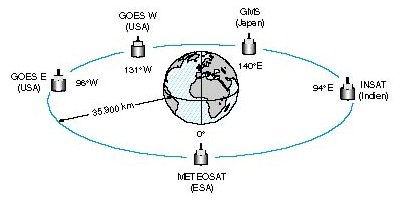
\includegraphics[width=0.5\linewidth]{images/Meteosat_geosats.jpg}
%     \caption{\footnotesize{Five identical geostationary satellites are arranged in a constellation along the equator. These include Meteosat (ESA), Himawari (JAXA), INSAT (ISRO), and GOES-E / GOES-W (NOAA). Together, they provide new images of global weather conditions every half hour, excluding the Polar Regions \cite{_esa_2013}.}}
%     \label{fig:Meteosat_geosats}
% \end{figure}
% \begin{figure}[H]
%     \centering
%     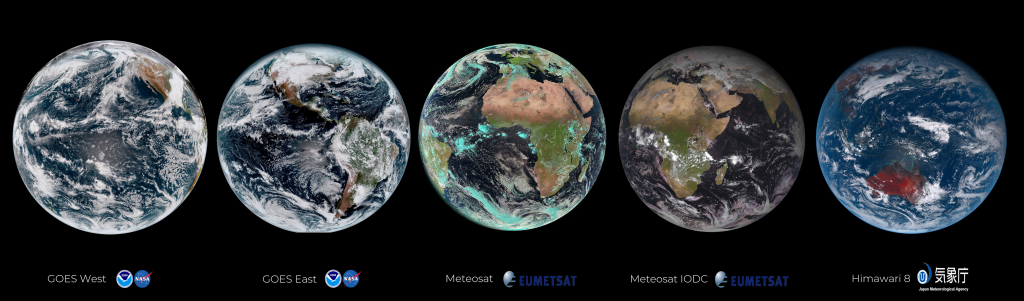
\includegraphics[width=0.8\linewidth]{images/full_earth_disk_image_GOES16_18_Meteosat11_9_Himawari9.png}
%     \caption{\footnotesize{Earth's full disk image by the geostationary satellite capable of fire detection. GOES W \& E, Meteosat 9 \& 11, Himawai 9.\cite{_algorithm_} }}
%     \label{fig:earth_full_disk_geosats}
% \end{figure}
\begin{figure}
    \centering
    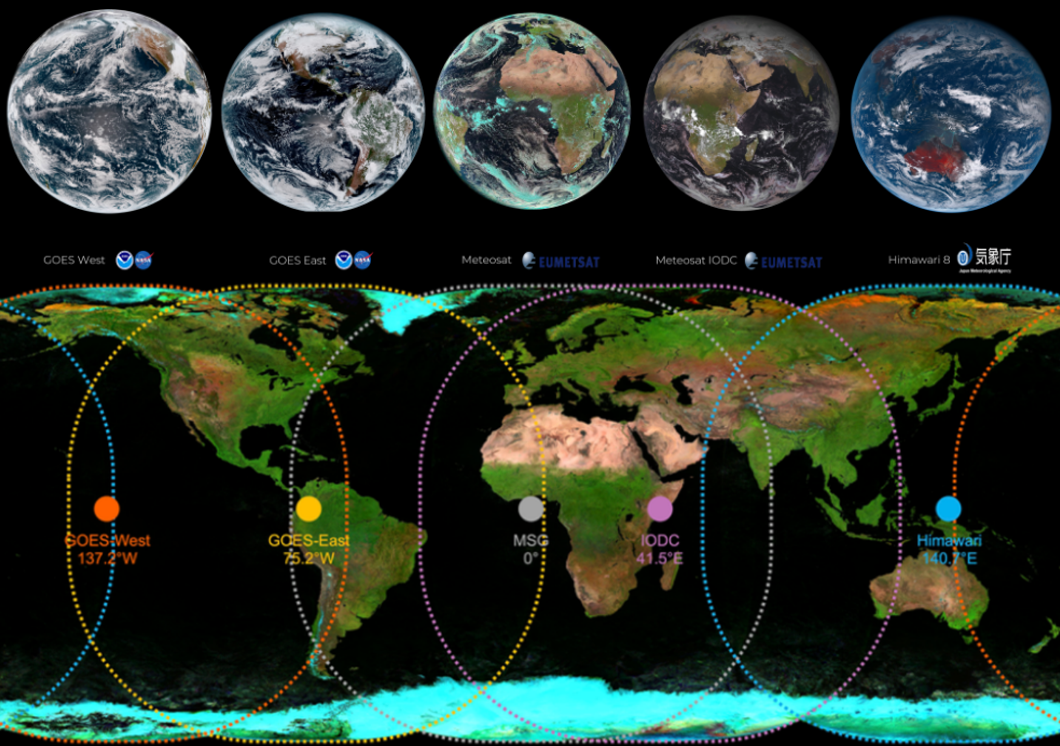
\includegraphics[width=1\linewidth]{images/FIRMS_GEO_sats_Earth_Disks.png}
    \caption{\footnotesize{Top: Earth's full disk image by the geostationary satellite capable of fire detection. GOES W \& E, Meteosat 9 \& 11, Himawai 9.\cite{_algorithm_} Bottom: Spatial coverage of five geostationary satellites used to achieve near real-time (10--15 min) active fire detection in FIRMS. This is the dataset used to populate the reference active fire events $\Upsilon_{ref}$ belonging to the global study temporal domain $\mathcal{T}_{global}$ \cite{davies_geostationary_2024}.}}
    \label{fig:firms_geostationary_sats}
\end{figure}


This multi-satellite geostationary constellation layer (GeoLayer) provides global coverage with a temporal resolution of $\Delta t_{FireDS} \approx 10-15$ minutes; . This high-cadence system captures the evolution of fire intensity, serving as the necessary "High-Frequency Ground Truth" to validate whether the proposed LEO constellation layer architecture (LeoLayer) successfully captures the fire timeline during its active phase; \inlineReq{R21}.

\begin{table}
\centering
\caption{\footnotesize{Composition of the Global Reference Data Source (FIRMS Geostationary). These instruments define the "True Events" ($\Psi_n$) used to validate the simulation in the 2024 temporal window.}}
\label{tab:geo_satellites}
\renewcommand{\arraystretch}{1.2}
\begin{tabular}{l l l c}
\toprule
\textbf{Satellite Platform} & \textbf{Instrument} & \textbf{Coverage Area} & \textbf{Resolution ($\Delta t$)} \\
\midrule
\textbf{GOES-16} (East) & ABI & North/South America (East) & 10 min \\
\textbf{GOES-18} (West) & ABI & North/South America (West) & 10 min \\
\textbf{Meteosat-9/11} & SEVIRI & Europe, Africa, Indian Ocean & 15 min \\
\textbf{Himawari-8/9} & AHI & Asia, Pacific, Australia & 10 min \\
\bottomrule
\end{tabular}
\end{table}


\paragraph{GeoLayer Spatial Resolution and Geometry Considerations} 
\label{sec:geolayer_spatial_and_temporal_resolution}

While the GeoLayer FIRMS$_{FireDS}$ dataset provides near-real-time active-fire reference data, it imposes specific spatial constraints that must be accounted for. The nominal spatial resolution at the sub-satellite point (nadir) ranges from $GSD_{GeoLayer} \approx$ 2 km to 3 km, which is significantly coarser than that of LEO sensors like VIIRS (375 m) or the desired constellation spatial resolution of 6 m/pixel \reqRef{R7}; \inlineReq{R22}. Furthermore, at the large viewing angles of geostationary orbits, the pixel footprint undergoes geometric distortion, increasing substantially toward the poles \cite{davies_geostationary_2024}.

However, for the specific purpose of this mission analysis—validating the temporal detection latency—this coarse spatial resolution is not a limiting factor. The typical field of view (FOV) and footprint (swath) of the proposed LEO CubeSat sensors significantly exceed the uncertainty associated with a single geostationary pixel ($\text{Swath}_{LEO} \gg GSD_{GeoLayer}$). Thus, even if the exact sub-pixel location of the fire is unknown within the 2–4 km footprint, the event remains well-contained within the observational swath of the passing satellite. Therefore, the geostationary fast-but-coarse detection remains a valid ground truth for assessing whether the constellation intercepted the region during the active fire window.

\begin{figure}[H]
    \centering
    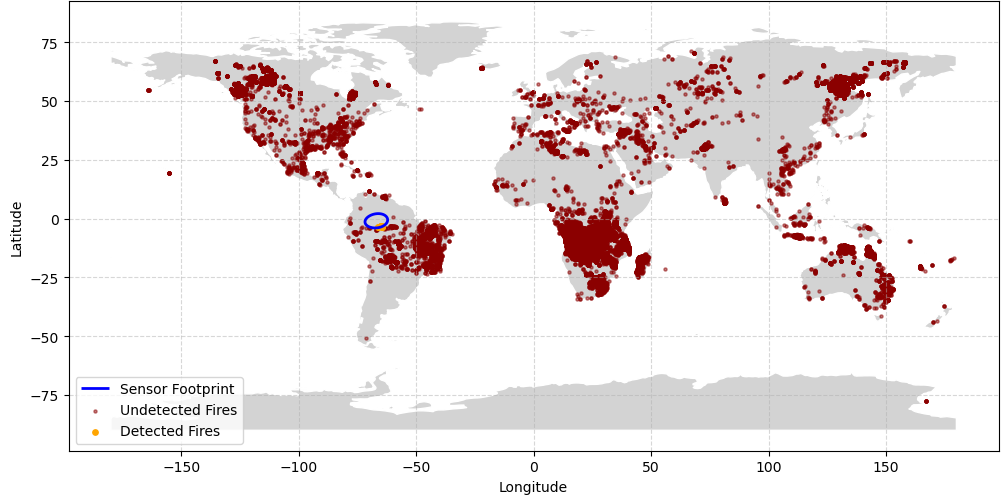
\includegraphics[width=1\linewidth]{images/map_viirs_active_fire_satellite_footprin_detection.png}
    \caption{\footnotesize{\textbf{Global distribution of Reference Fire Events ($\Upsilon_{ref}$) for 2024.} 
    The map illustrates the spatial aggregation of all active fire detections $\Psi_n$ derived from the FIRMS Geostationary dataset (GOES, Meteosat, Himawari) throughout the observation window $\mathcal{T}_{global}$. These discrete high-cadence events serve as the empirical ground truth for validating the constellation's detection latency.}}
    \label{fig:firms_geo_2024}
\end{figure}

\subparagraph{GeoLayer as Candidate Architectural Component} 
\label{sec:geolayer_candidate_architecture}
\hspace{0pt}

Beyond serving as a validation baseline, the high temporal cadence of the \textit{GeoLayer} also highlights its potential utility as an operational segment of the mission. Integrating these coarse GeoLayer rapid-fire alerts with the high-resolution capabilities of the \textit{LeoLayer} enables a viable "Tip-and-Cue" architecture strategy; \inlineReq{R23}. This cooperative multi-sensor layered approach, takes advantage of available public infrastructure (GeoLayer), providing a pathway to simultaneously satisfy the demanding, often conflicting requirements of rapid global revisit ($t_{revisit} \approx 30$ min) and high spatial detail ($GSD \approx 6$ m); see \reqRef{R7}, \reqRef{R8}. Therefore, the satellites indicated in table \ref{tab:geo_satellites}, which compose the FIRMS fire-alert, are identified as candidates for the GeoLayer architecture component for a global domain mission solution \inlineReq{24}. The formal trade-off analysis and detailed design of this hybrid architecture are presented in the Mission Architecture section.

\begin{figure}[H]
    \centering
    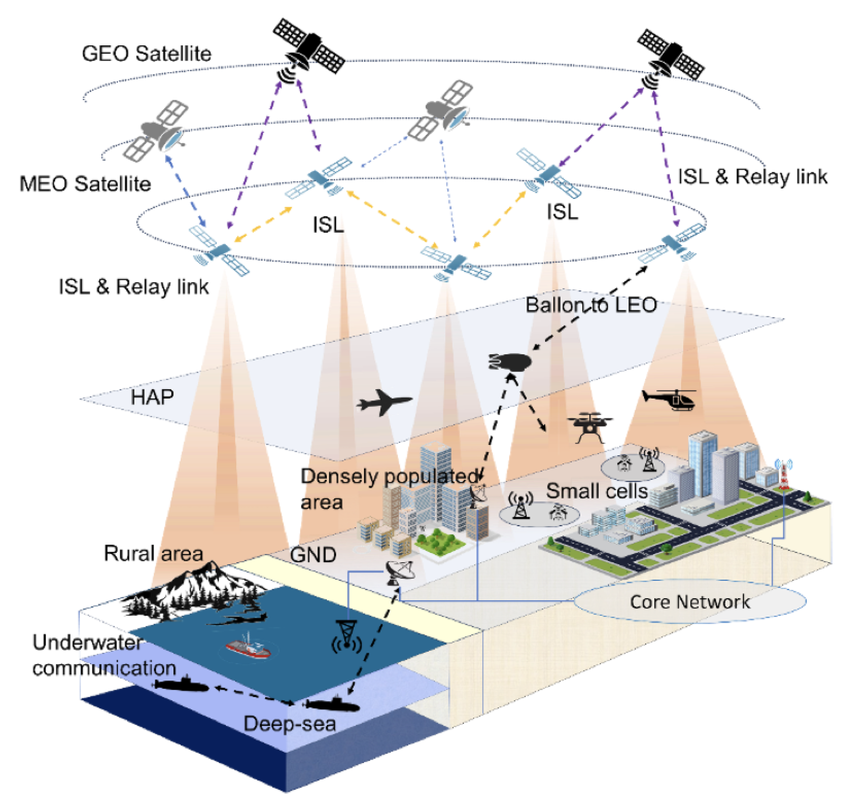
\includegraphics[width=0.85\linewidth]{images/tip-and-cue_architecture_example.png}
    \caption{\footnotesize{Example of tip-and-cue satellite communication architecture. Each sensor has unique advantages and disadvantages; combining and communicating these systems leads to higher temporo-spatial fidelity solutions impossible with separated units~\cite{_architecture_tipcue}.}}
    \label{fig:tip-and-cue_example}
\end{figure}

\subparagraph{GeoLayer New Generation Satellites} \hspace{0pt}
\label{sec:geolayer_new_gen}

New-generation geostationary satellites are emerging, improving spatial resolution and temporal detection capabilities. An example is \textbf{Meteosat-12} (formerly MTG-I1), the first of the Meteosat Third Generation Imager series. Declared fully operational in December 2024, this platform carries the Flexible Combined Imager (FCI), which enhances spatial resolution over Europe to \textbf{0.5 km - 2 km}, a marked improvement compared to the 3 km standard of the previous generation (MSG, GOES) \cite{_meteosat_2022}. 

\begin{figure}[H]
    \centering
    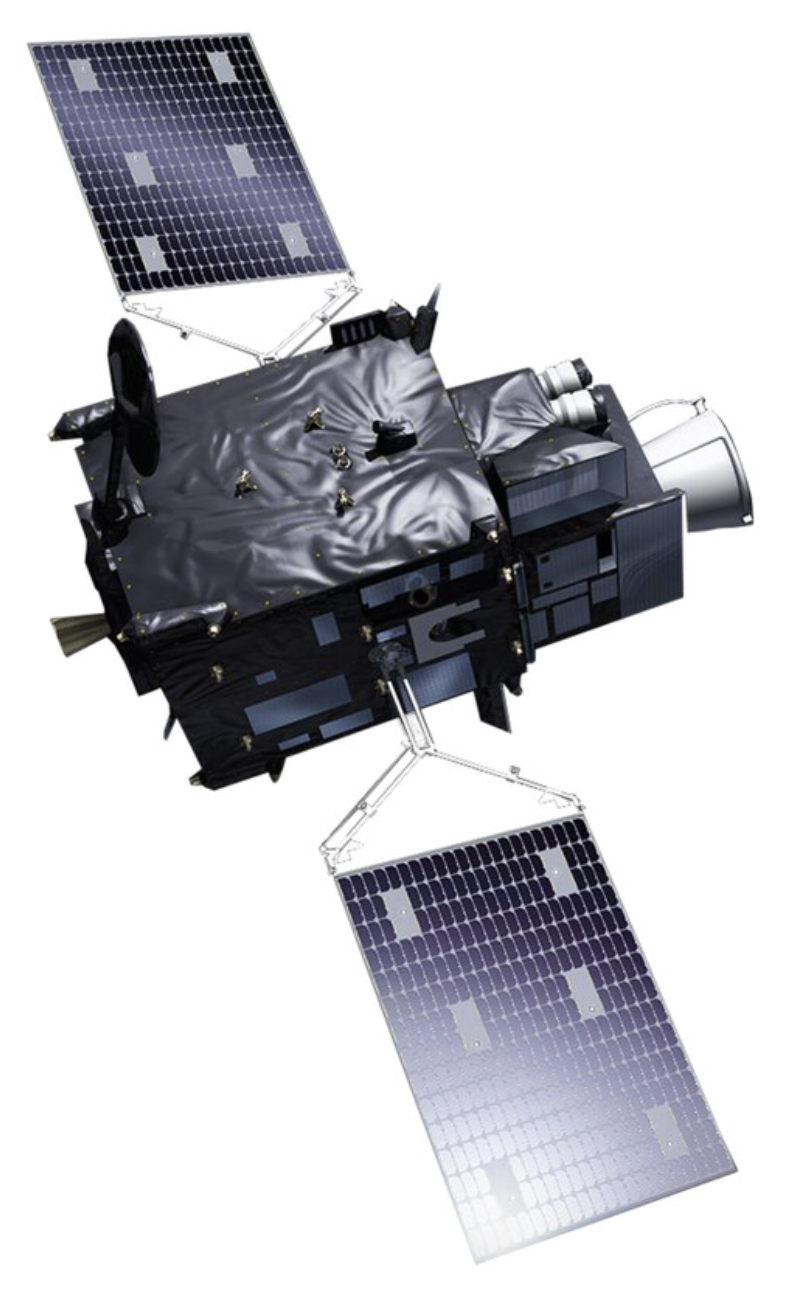
\includegraphics[width=0.15\linewidth]{images/meteosat12_render.png}
    \caption{\footnotesize{Meteosat-12,  Third Generation Geostationary Imager capable of 2.5min scan over European section with\textbf{ \textbf{0.5 km - 2 km}} GSD}}
    \label{fig:meteosat12_render}
\end{figure}

Furthermore, the MTG-I platform architecture introduces the capability for a \textbf{Rapid Scan Service (RSS)} of the European sector (Northern Quarter of Earth's disk) every \textbf{2.5 minutes} with all 16 spectral channels, significantly faster than the standard 10-minute Full Disk Scan \cite{eumetsat_rss_info, eumetsat_rss_2024}. The system also supports fire alerts and Fire Radiative Power (FRP) products, offering superior sensitivity for early event detection. 

\begin{figure}[H]
    \centering
    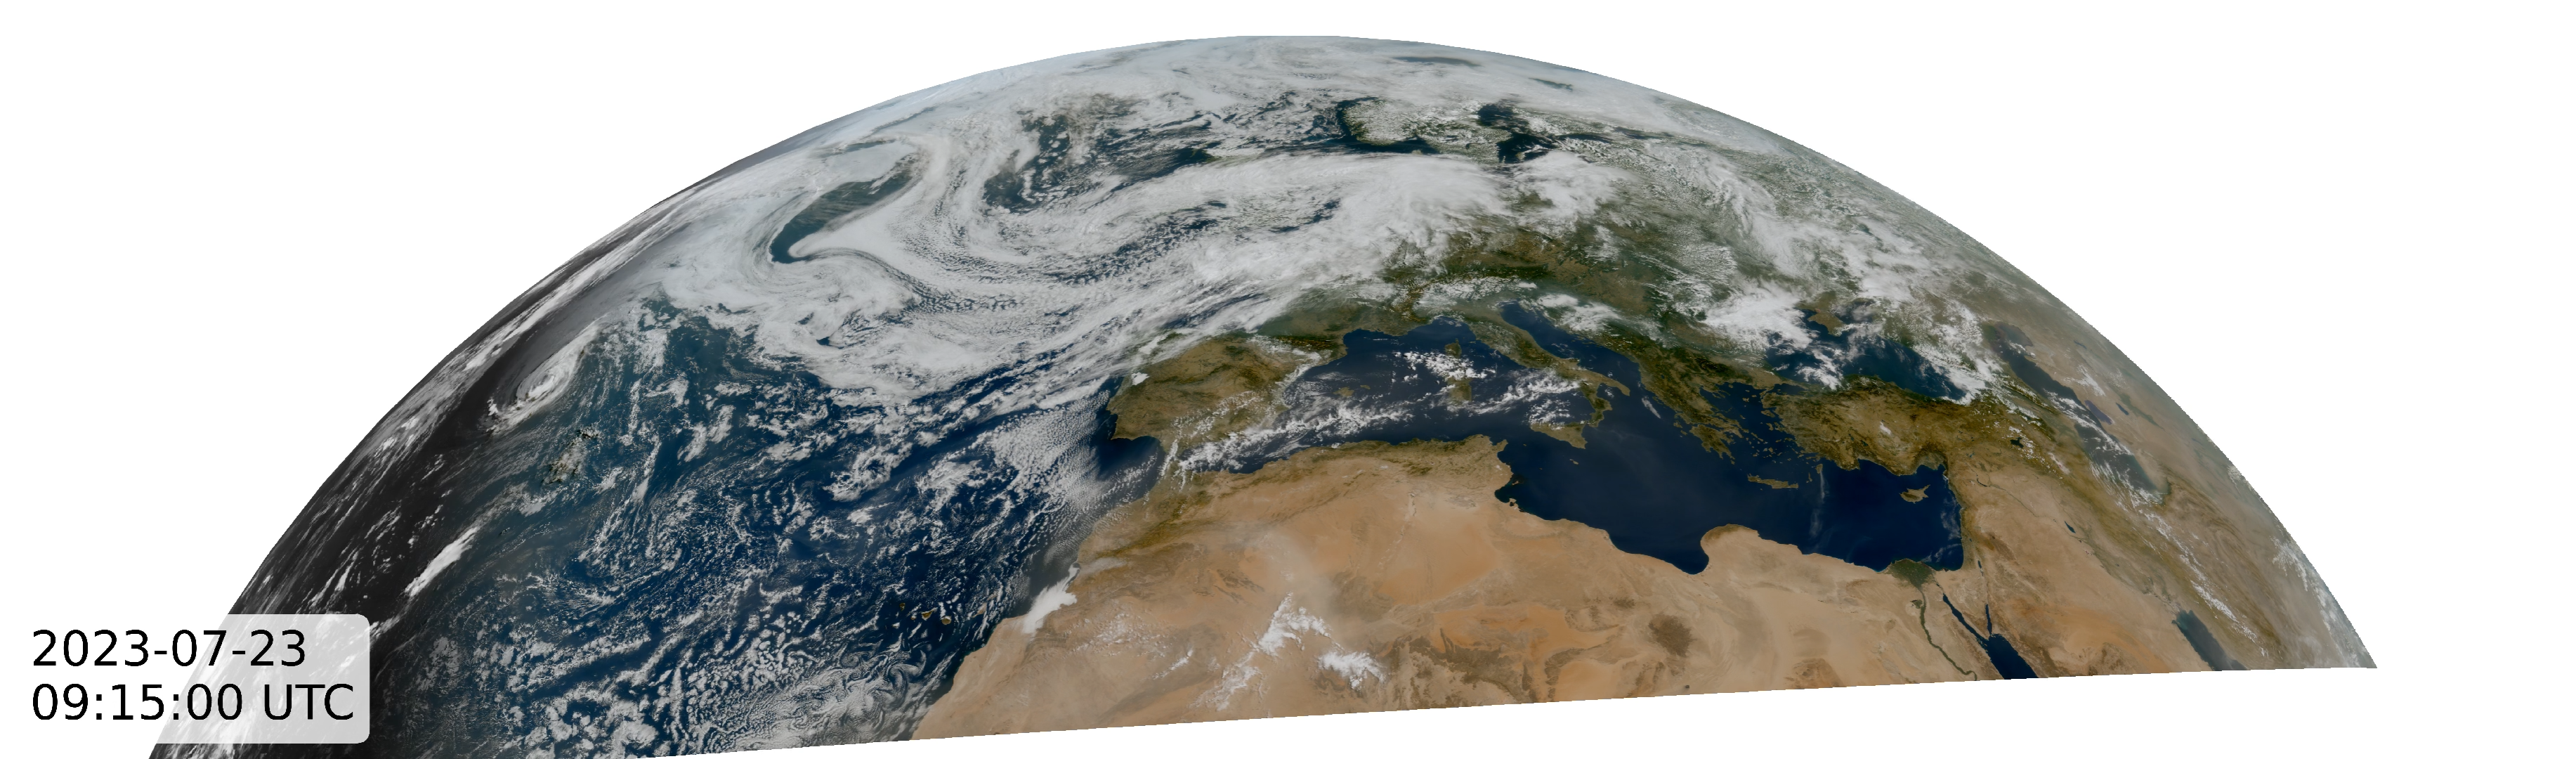
\includegraphics[width=1\linewidth]{images/meteosat12_rapid_scan_service_example.png}
    \caption{\footnotesize{Meteosat-12 Rapid Scan Service test dataset example. FCI True Colour RGB with night layer, animation with 2.5min repeat rate, 23 July 2023, 08:52:30 UTC-24 July 2023, 07:57:30 UTC Enter Caption. Video at \cite{eumetsat_rss_info}. }}
    \label{fig:meteosat12_rss}
\end{figure}

Looking ahead, the constellation will be completed by \textbf{Meteosat-14} (MTG-I2), which is scheduled for launch in \textbf{September 2026} \cite{eumetsat_planned_launches}. Following its commissioning, this platform will solidify the high-cadence architecture by assuming responsibility for the dedicated Rapid Scan Service (RSS) from the legacy fleet in \textbf{2027}.

Given these performance metrics, Meteosat-12 \& 14 are identified as strong candidates for the GeoLayer component over Europe \inlineReq{25}. However, a unified global dataset for this new, higher-fidelity geosat generation, spanning longitudes worldwide, does not yet exist. Therefore, for global performance analysis in this work, we will continue to use the established FIRMS Geolayer FIRMS$_{FireDS}$ dataset, which provides the global consistency required for the simulation.

%%% ----- Continue working


\section{Requirements Study Case Summary and Chapter Conclusion}
\label{sec:requirements-study-case-summary}

This section consolidates the study domain definitions from the preceding sections into traceable, design-level requirements. These requirements establish the spatial and temporal boundaries for the mission simulation, define the reference datasets for verification, and specify the architectural constraints for the satellite constellation assessment.

Detailed requirements derived in this chapter (R9--R25), covering the Core Study Domain, Global Study Domain, Reference Data, and Architecture constraints, are provided in Appendix~\ref{sec:app_req_ch2}.

In summary, this chapter has defined the two observational study domains that anchor the mission analysis. The Core Study Domain $\mathcal{D}_{core}$ fixes the spatial boundaries to mainland Portugal and the temporal bounds to its fire season centred on the August~18 peak, providing the primary evaluation context for the constellation. The Global Study Domain $\mathcal{D}_{global}$ extends coverage to all fire-prone regions classified by climate regime and fire frequency, using the FIRMS geostationary active-fire dataset as an observation-based, high-cadence verification baseline. Together, the spatial, temporal, and data-source definitions consolidated in requirements R9--R25 establish the inputs for the physical foundations of fire remote sensing developed in the next chapter.
